\subsection{Qualitative}
\label{subsec:experiments-qualitative}

\def\BSDSCroppedScale{0.25}
\def\SBDCroppedScale{0.3}
\def\FashCroppedScale{0.195}
\begin{figure*}
	\centering
	\vspace{-0.5cm}
	% W %%%%%%%%%%%%%%%%%%%%%%%%%%%%%%%%%%%%%%%%%%%%%%%%%%%%%%%%%%%%%%%%%%%%%%%%
	\begin{subfigure}[b]{0.02\textwidth}
		\rotatebox{90}{\small\hphantom{aaai}\W}
	\end{subfigure}
	\begin{subfigure}[b]{0.16\textwidth}
        \begin{center}
            \BSDS
        \end{center}
        \vskip -6px
		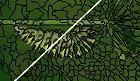
\includegraphics[height=1.65cm]{pictures/bsds500/w/cropped/w_35028_contours}
	\end{subfigure}
	\begin{subfigure}[b]{0.129\textwidth}
        \begin{center}
            \SBD
        \end{center}
        \vskip -6px
		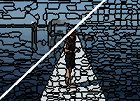
\includegraphics[height=1.65cm]{pictures/sbd/w/cropped/w_0004774_contours}
	\end{subfigure}
	\begin{subfigure}[b]{0.10\textwidth}
        \begin{center}
            \Fash
        \end{center}
        \vskip -6px
		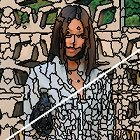
\includegraphics[height=1.65cm]{pictures/fash/w/cropped/w_010_contours}
	\end{subfigure}
	% EAMS %%%%%%%%%%%%%%%%%%%%%%%%%%%%%%%%%%%%%%%%%%%%%%%%%%%%%%%%%%%%%%%%%%%%%
	\begin{subfigure}[b]{0.02\textwidth}
		\rotatebox{90}{\small\hphantom{ai}\EAMS}
	\end{subfigure}
	\begin{subfigure}[b]{0.16\textwidth}
        \begin{center}
            \BSDS
        \end{center}
        \vskip -6px
		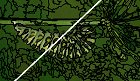
\includegraphics[height=1.65cm]{pictures/bsds500/eams/cropped/eams_35028_contours}
	\end{subfigure}
	\begin{subfigure}[b]{0.129\textwidth}
        \begin{center}
            \SBD
        \end{center}
        \vskip -6px
		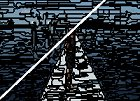
\includegraphics[height=1.65cm]{pictures/sbd/eams/cropped/eams_0004774_contours}
	\end{subfigure}
	\begin{subfigure}[b]{0.10\textwidth}
        \begin{center}
            \Fash
        \end{center}
        \vskip -6px
		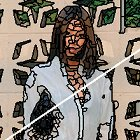
\includegraphics[height=1.65cm]{pictures/fash/eams/cropped/eams_010_contours}
	\end{subfigure}\\
	% NC %%%%%%%%%%%%%%%%%%%%%%%%%%%%%%%%%%%%%%%%%%%%%%%%%%%%%%%%%%%%%%%%%%%%%%%
	\begin{subfigure}[b]{0.02\textwidth}
		\rotatebox{90}{\small\hphantom{aaa}\NC}
	\end{subfigure}
	\begin{subfigure}[b]{0.16\textwidth}
		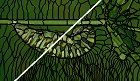
\includegraphics[height=1.65cm]{pictures/bsds500/nc/cropped/nc_35028_contours}
	\end{subfigure}
	\begin{subfigure}[b]{0.129\textwidth}
		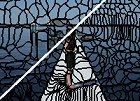
\includegraphics[height=1.65cm]{pictures/sbd/nc/cropped/nc_0004774_contours}
	\end{subfigure}
	\begin{subfigure}[b]{0.10\textwidth}
		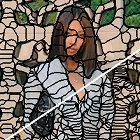
\includegraphics[height=1.65cm]{pictures/fash/nc/cropped/nc_010_contours}
	\end{subfigure}
	% FH %%%%%%%%%%%%%%%%%%%%%%%%%%%%%%%%%%%%%%%%%%%%%%%%%%%%%%%%%%%%%%%%%%%%%%%
	\begin{subfigure}[b]{0.02\textwidth}
		\rotatebox{90}{\small\hphantom{aaa}\FH}
	\end{subfigure}
	\begin{subfigure}[b]{0.16\textwidth}
		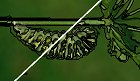
\includegraphics[height=1.65cm]{pictures/bsds500/fh/cropped/fh_35028_contours}
	\end{subfigure}
	\begin{subfigure}[b]{0.129\textwidth}
		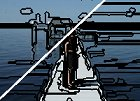
\includegraphics[height=1.65cm]{pictures/sbd/fh/cropped/fh_0004774_contours}
	\end{subfigure}
	\begin{subfigure}[b]{0.10\textwidth}
		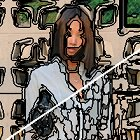
\includegraphics[height=1.65cm]{pictures/fash/fh/cropped/fh_010_contours}
	\end{subfigure}\\
	% RW %%%%%%%%%%%%%%%%%%%%%%%%%%%%%%%%%%%%%%%%%%%%%%%%%%%%%%%%%%%%%%%%%%%%%%%
	\begin{subfigure}[b]{0.02\textwidth}
		\rotatebox{90}{\small\hphantom{aaa}\RW}
	\end{subfigure}
	\begin{subfigure}[b]{0.16\textwidth}
		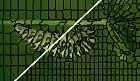
\includegraphics[height=1.65cm]{pictures/bsds500/rw/cropped/rw_35028_contours}
	\end{subfigure}
	\begin{subfigure}[b]{0.129\textwidth}
		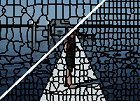
\includegraphics[height=1.65cm]{pictures/sbd/rw/cropped/rw_0004774_contours}
	\end{subfigure}
	\begin{subfigure}[b]{0.10\textwidth}
		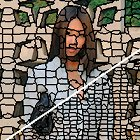
\includegraphics[height=1.65cm]{pictures/fash/rw/cropped/rw_010_contours}
	\end{subfigure}
	% QS %%%%%%%%%%%%%%%%%%%%%%%%%%%%%%%%%%%%%%%%%%%%%%%%%%%%%%%%%%%%%%%%%%%%%%%
	\begin{subfigure}[b]{0.02\textwidth}
		\rotatebox{90}{\small\hphantom{aaa}\QS}
	\end{subfigure}
	\begin{subfigure}[b]{0.16\textwidth}
		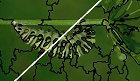
\includegraphics[height=1.65cm]{pictures/bsds500/qs/cropped/qs_35028_contours}
	\end{subfigure}
	\begin{subfigure}[b]{0.129\textwidth}
		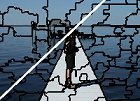
\includegraphics[height=1.65cm]{pictures/sbd/qs/cropped/qs_0004774_contours}
	\end{subfigure}
	\begin{subfigure}[b]{0.10\textwidth}
		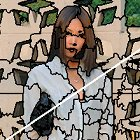
\includegraphics[height=1.65cm]{pictures/fash/qs/cropped/qs_010_contours}
	\end{subfigure}\\
	% PF %%%%%%%%%%%%%%%%%%%%%%%%%%%%%%%%%%%%%%%%%%%%%%%%%%%%%%%%%%%%%%%%%%%%%%%
	\begin{subfigure}[b]{0.02\textwidth}
		\rotatebox{90}{\small\hphantom{aaa}\PF}
	\end{subfigure}
	\begin{subfigure}[b]{0.16\textwidth}
		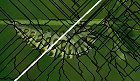
\includegraphics[height=1.65cm]{pictures/bsds500/pf/cropped/pf_35028_contours}
	\end{subfigure}
	\begin{subfigure}[b]{0.129\textwidth}
		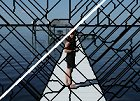
\includegraphics[height=1.65cm]{pictures/sbd/pf/cropped/pf_0004774_contours}
	\end{subfigure}
	\begin{subfigure}[b]{0.10\textwidth}
		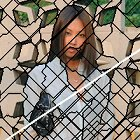
\includegraphics[height=1.65cm]{pictures/fash/pf/cropped/pf_010_contours}
	\end{subfigure}
	% TP %%%%%%%%%%%%%%%%%%%%%%%%%%%%%%%%%%%%%%%%%%%%%%%%%%%%%%%%%%%%%%%%%%%%%%%
	\begin{subfigure}[b]{0.02\textwidth}
		\rotatebox{90}{\small\hphantom{aaa}\TP}
	\end{subfigure}
	\begin{subfigure}[b]{0.16\textwidth}
		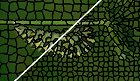
\includegraphics[height=1.65cm]{pictures/bsds500/tp/cropped/tp_35028_contours}
	\end{subfigure}
	\begin{subfigure}[b]{0.129\textwidth}
		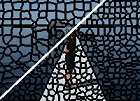
\includegraphics[height=1.65cm]{pictures/sbd/tp/cropped/tp_0004774_contours}
	\end{subfigure}
	\begin{subfigure}[b]{0.10\textwidth}
		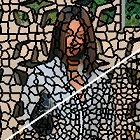
\includegraphics[height=1.65cm]{pictures/fash/tp/cropped/tp_010_contours}
	\end{subfigure}\\
	% CIS %%%%%%%%%%%%%%%%%%%%%%%%%%%%%%%%%%%%%%%%%%%%%%%%%%%%%%%%%%%%%%%%%%%%%%
	\begin{subfigure}[b]{0.02\textwidth}
		\rotatebox{90}{\small\hphantom{aai}\CIS}
	\end{subfigure}
	\begin{subfigure}[b]{0.16\textwidth}
		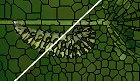
\includegraphics[height=1.65cm]{pictures/bsds500/cis/cropped/cis_35028_contours}
	\end{subfigure}
	\begin{subfigure}[b]{0.129\textwidth}
		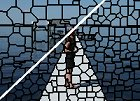
\includegraphics[height=1.65cm]{pictures/sbd/cis/cropped/cis_0004774_contours}
	\end{subfigure}
	\begin{subfigure}[b]{0.10\textwidth}
		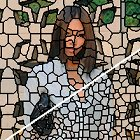
\includegraphics[height=1.65cm]{pictures/fash/cis/cropped/cis_010_contours}
	\end{subfigure}
	% SLIC %%%%%%%%%%%%%%%%%%%%%%%%%%%%%%%%%%%%%%%%%%%%%%%%%%%%%%%%%%%%%%%%%%%%%
	\begin{subfigure}[b]{0.02\textwidth}
		\rotatebox{90}{\small\hphantom{aa}\SLIC}
	\end{subfigure}
	\begin{subfigure}[b]{0.16\textwidth}
		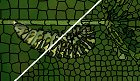
\includegraphics[height=1.65cm]{pictures/bsds500/slic/cropped/slic_35028_contours}
	\end{subfigure}
	\begin{subfigure}[b]{0.129\textwidth}
		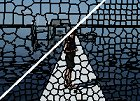
\includegraphics[height=1.65cm]{pictures/sbd/slic/cropped/slic_0004774_contours}
	\end{subfigure}
	\begin{subfigure}[b]{0.10\textwidth}
		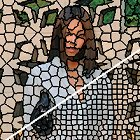
\includegraphics[height=1.65cm]{pictures/fash/slic/cropped/slic_010_contours}
	\end{subfigure}\\
	% CRS %%%%%%%%%%%%%%%%%%%%%%%%%%%%%%%%%%%%%%%%%%%%%%%%%%%%%%%%%%%%%%%%%%%%%%
	\begin{subfigure}[b]{0.02\textwidth}
		\rotatebox{90}{\small\hphantom{aai}\CRS}
	\end{subfigure}
	\begin{subfigure}[b]{0.16\textwidth}
		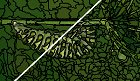
\includegraphics[height=1.65cm]{pictures/bsds500/crs/cropped/crs_35028_contours}
	\end{subfigure}
	\begin{subfigure}[b]{0.129\textwidth}
		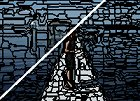
\includegraphics[height=1.65cm]{pictures/sbd/crs/cropped/crs_0004774_contours}
	\end{subfigure}
	\begin{subfigure}[b]{0.10\textwidth}
		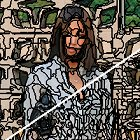
\includegraphics[height=1.65cm]{pictures/fash/crs/cropped/crs_010_contours}
	\end{subfigure}
	% ERS %%%%%%%%%%%%%%%%%%%%%%%%%%%%%%%%%%%%%%%%%%%%%%%%%%%%%%%%%%%%%%%%%%%%%%
	\begin{subfigure}[b]{0.02\textwidth}
		\rotatebox{90}{\small\hphantom{aai}\ERS}
	\end{subfigure}
	\begin{subfigure}[b]{0.16\textwidth}
		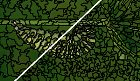
\includegraphics[height=1.65cm]{pictures/bsds500/ers/cropped/ers_35028_contours}
	\end{subfigure}
	\begin{subfigure}[b]{0.129\textwidth}
		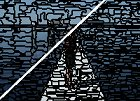
\includegraphics[height=1.65cm]{pictures/sbd/ers/cropped/ers_0004774_contours}
	\end{subfigure}
	\begin{subfigure}[b]{0.10\textwidth}
		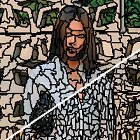
\includegraphics[height=1.65cm]{pictures/fash/ers/cropped/ers_010_contours}
	\end{subfigure}\\
	% PB %%%%%%%%%%%%%%%%%%%%%%%%%%%%%%%%%%%%%%%%%%%%%%%%%%%%%%%%%%%%%%%%%%%%%%
	\begin{subfigure}[b]{0.02\textwidth}
		\rotatebox{90}{\small\hphantom{aaa}\PB}
	\end{subfigure}
	\begin{subfigure}[b]{0.16\textwidth}
		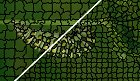
\includegraphics[height=1.65cm]{pictures/bsds500/pb/cropped/pb_35028_contours}
	\end{subfigure}
	\begin{subfigure}[b]{0.129\textwidth}
		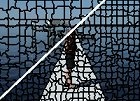
\includegraphics[height=1.65cm]{pictures/sbd/pb/cropped/pb_0004774_contours}
	\end{subfigure}
	\begin{subfigure}[b]{0.10\textwidth}
		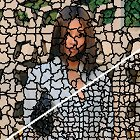
\includegraphics[height=1.65cm]{pictures/fash/pb/cropped/pb_010_contours}
	\end{subfigure}
	% SEEDS %%%%%%%%%%%%%%%%%%%%%%%%%%%%%%%%%%%%%%%%%%%%%%%%%%%%%%%%%%%%%%%%%%%%%%
	\begin{subfigure}[b]{0.02\textwidth}
		\rotatebox{90}{\small\hphantom{a}\SEEDS}
	\end{subfigure}
	\begin{subfigure}[b]{0.16\textwidth}
		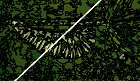
\includegraphics[height=1.65cm]{pictures/bsds500/seeds/cropped/seeds_35028_contours}
	\end{subfigure}
	\begin{subfigure}[b]{0.129\textwidth}
		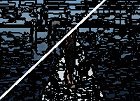
\includegraphics[height=1.65cm]{pictures/sbd/seeds/cropped/seeds_0004774_contours}
	\end{subfigure}
	\begin{subfigure}[b]{0.10\textwidth}
		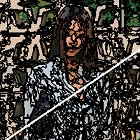
\includegraphics[height=1.65cm]{pictures/fash/seeds/cropped/seeds_010_contours}
	\end{subfigure}\\
	% TPS %%%%%%%%%%%%%%%%%%%%%%%%%%%%%%%%%%%%%%%%%%%%%%%%%%%%%%%%%%%%%%%%%%%%%%
	\begin{subfigure}[b]{0.02\textwidth}
		\rotatebox{90}{\small\hphantom{aai}\TPS}
	\end{subfigure}
	\begin{subfigure}[b]{0.16\textwidth}
		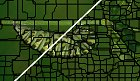
\includegraphics[height=1.65cm]{pictures/bsds500/tps/cropped/tps_35028_contours}
	\end{subfigure}
	\begin{subfigure}[b]{0.129\textwidth}
		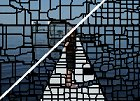
\includegraphics[height=1.65cm]{pictures/sbd/tps/cropped/tps_0004774_contours}
	\end{subfigure}
	\begin{subfigure}[b]{0.10\textwidth}
		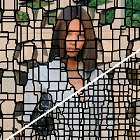
\includegraphics[height=1.65cm]{pictures/fash/tps/cropped/tps_010_contours}
	\end{subfigure}
	% VC %%%%%%%%%%%%%%%%%%%%%%%%%%%%%%%%%%%%%%%%%%%%%%%%%%%%%%%%%%%%%%%%%%%%%%
	\begin{subfigure}[b]{0.02\textwidth}
		\rotatebox{90}{\small\hphantom{aaa}\VC}
	\end{subfigure}
	\begin{subfigure}[b]{0.16\textwidth}
		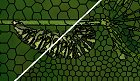
\includegraphics[height=1.65cm]{pictures/bsds500/vc/cropped/vc_35028_contours}
	\end{subfigure}
	\begin{subfigure}[b]{0.129\textwidth}
		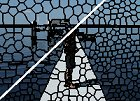
\includegraphics[height=1.65cm]{pictures/sbd/vc/cropped/vc_0004774_contours}
	\end{subfigure}
	\begin{subfigure}[b]{0.10\textwidth}
		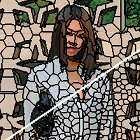
\includegraphics[height=1.65cm]{pictures/fash/vc/cropped/vc_010_contours}
	\end{subfigure}\\
	% CCS %%%%%%%%%%%%%%%%%%%%%%%%%%%%%%%%%%%%%%%%%%%%%%%%%%%%%%%%%%%%%%%%%%%%%%
	\begin{subfigure}[b]{0.02\textwidth}
		\rotatebox{90}{\small\hphantom{aai}\CCS}
	\end{subfigure}
	\begin{subfigure}[b]{0.16\textwidth}
		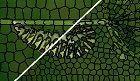
\includegraphics[height=1.65cm]{pictures/bsds500/ccs/cropped/ccs_35028_contours}
	\end{subfigure}
	\begin{subfigure}[b]{0.129\textwidth}
		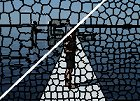
\includegraphics[height=1.65cm]{pictures/sbd/ccs/cropped/ccs_0004774_contours}
	\end{subfigure}
	\begin{subfigure}[b]{0.10\textwidth}
		\includegraphics[height=1.65cm]{pictures/fash/ccs/cropped/ccs_010_contours}
	\end{subfigure}
	% CW %%%%%%%%%%%%%%%%%%%%%%%%%%%%%%%%%%%%%%%%%%%%%%%%%%%%%%%%%%%%%%%%%%%%%%
	\begin{subfigure}[b]{0.02\textwidth}
		\rotatebox{90}{\small\hphantom{aaa}\CW}
	\end{subfigure}
	\begin{subfigure}[b]{0.16\textwidth}
		\includegraphics[height=1.65cm]{pictures/bsds500/cw/cropped/cw_35028_contours}
	\end{subfigure}
	\begin{subfigure}[b]{0.129\textwidth}
		\includegraphics[height=1.65cm]{pictures/sbd/cw/cropped/cw_0004774_contours}
	\end{subfigure}
	\begin{subfigure}[b]{0.10\textwidth}
		\includegraphics[height=1.65cm]{pictures/fash/cw/cropped/cw_010_contours}
	\end{subfigure}\\
	% ERGC %%%%%%%%%%%%%%%%%%%%%%%%%%%%%%%%%%%%%%%%%%%%%%%%%%%%%%%%%%%%%%%%%%%%%%
	\begin{subfigure}[b]{0.02\textwidth}
		\rotatebox{90}{\small\hphantom{aa}\ERGC}
	\end{subfigure}
	\begin{subfigure}[b]{0.16\textwidth}
		\includegraphics[height=1.65cm]{pictures/bsds500/ergc/cropped/ergc_35028_contours}
	\end{subfigure}
	\begin{subfigure}[b]{0.129\textwidth}
		\includegraphics[height=1.65cm]{pictures/sbd/ergc/cropped/ergc_0004774_contours}
	\end{subfigure}
	\begin{subfigure}[b]{0.10\textwidth}
		\includegraphics[height=1.65cm]{pictures/fash/ergc/cropped/ergc_010_contours}
	\end{subfigure}
	% MSS %%%%%%%%%%%%%%%%%%%%%%%%%%%%%%%%%%%%%%%%%%%%%%%%%%%%%%%%%%%%%%%%%%%%%%
	\begin{subfigure}[b]{0.02\textwidth}
		\rotatebox{90}{\small\hphantom{aai}\MSS}
	\end{subfigure}
	\begin{subfigure}[b]{0.16\textwidth}
		\includegraphics[height=1.65cm]{pictures/bsds500/mss/cropped/mss_35028_contours}
	\end{subfigure}
	\begin{subfigure}[b]{0.129\textwidth}
		\includegraphics[height=1.65cm]{pictures/sbd/mss/cropped/mss_0004774_contours}
	\end{subfigure}
	\begin{subfigure}[b]{0.10\textwidth}
		\includegraphics[height=1.65cm]{pictures/fash/mss/cropped/mss_010_contours}
	\end{subfigure}\\
	% preSLIC %%%%%%%%%%%%%%%%%%%%%%%%%%%%%%%%%%%%%%%%%%%%%%%%%%%%%%%%%%%%%%%%%%%%%%
	\begin{subfigure}[b]{0.02\textwidth}
		\rotatebox{90}{\small\hphantom{a}\preSLIC}
	\end{subfigure}
	\begin{subfigure}[b]{0.16\textwidth}
		\includegraphics[height=1.65cm]{pictures/bsds500/preslic/cropped/preslic_35028_contours}
	\end{subfigure}
	\begin{subfigure}[b]{0.129\textwidth}
		\includegraphics[height=1.65cm]{pictures/sbd/preslic/cropped/preslic_0004774_contours}
	\end{subfigure}
	\begin{subfigure}[b]{0.10\textwidth}
		\includegraphics[height=1.65cm]{pictures/fash/preslic/cropped/preslic_010_contours}
	\end{subfigure}
	% WP %%%%%%%%%%%%%%%%%%%%%%%%%%%%%%%%%%%%%%%%%%%%%%%%%%%%%%%%%%%%%%%%%%%%%%
	\begin{subfigure}[b]{0.02\textwidth}
		\rotatebox{90}{\small\hphantom{aaa}\WP}
	\end{subfigure}
	\begin{subfigure}[b]{0.16\textwidth}
		\includegraphics[height=1.65cm]{pictures/bsds500/wp/cropped/wp_35028_contours}
	\end{subfigure}
	\begin{subfigure}[b]{0.129\textwidth}
		\includegraphics[height=1.65cm]{pictures/sbd/wp/cropped/wp_0004774_contours}
	\end{subfigure}
	\begin{subfigure}[b]{0.10\textwidth}
		\includegraphics[height=1.65cm]{pictures/fash/wp/cropped/wp_010_contours}
	\end{subfigure}\\
	% ETPS %%%%%%%%%%%%%%%%%%%%%%%%%%%%%%%%%%%%%%%%%%%%%%%%%%%%%%%%%%%%%%%%%%%%%%
	\begin{subfigure}[b]{0.02\textwidth}
		\rotatebox{90}{\small\hphantom{aa}\ETPS}
	\end{subfigure}
	\begin{subfigure}[b]{0.16\textwidth}
		\includegraphics[height=1.65cm]{pictures/bsds500/etps/cropped/etps_35028_contours}
	\end{subfigure}
	\begin{subfigure}[b]{0.129\textwidth}
		\includegraphics[height=1.65cm]{pictures/sbd/etps/cropped/etps_0004774_contours}
	\end{subfigure}
	\begin{subfigure}[b]{0.10\textwidth}
		\includegraphics[height=1.65cm]{pictures/fash/etps/cropped/etps_010_contours}
	\end{subfigure}
	% LSC %%%%%%%%%%%%%%%%%%%%%%%%%%%%%%%%%%%%%%%%%%%%%%%%%%%%%%%%%%%%%%%%%%%%%%
	\begin{subfigure}[b]{0.02\textwidth}
		\rotatebox{90}{\small\hphantom{aai}\LSC}
	\end{subfigure}
	\begin{subfigure}[b]{0.16\textwidth}
		\includegraphics[height=1.65cm]{pictures/bsds500/lsc/cropped/lsc_35028_contours}
	\end{subfigure}
	\begin{subfigure}[b]{0.129\textwidth}
		\includegraphics[height=1.65cm]{pictures/sbd/lsc/cropped/lsc_0004774_contours}
	\end{subfigure}
	\begin{subfigure}[b]{0.10\textwidth}
		\includegraphics[height=1.65cm]{pictures/fash/lsc/cropped/lsc_010_contours}
	\end{subfigure}\\
	% POISE %%%%%%%%%%%%%%%%%%%%%%%%%%%%%%%%%%%%%%%%%%%%%%%%%%%%%%%%%%%%%%%%%%%%%%
	\begin{subfigure}[b]{0.02\textwidth}
		\rotatebox{90}{\small\hphantom{a}\POISE}
	\end{subfigure}
	\begin{subfigure}[b]{0.16\textwidth}
		\includegraphics[height=1.65cm]{pictures/bsds500/poise/cropped/poise_35028_contours}
	\end{subfigure}
	\begin{subfigure}[b]{0.129\textwidth}
		\includegraphics[height=1.65cm]{pictures/sbd/poise/cropped/poise_0004774_contours}
	\end{subfigure}
	\begin{subfigure}[b]{0.10\textwidth}
		\includegraphics[height=1.65cm]{pictures/fash/poise/cropped/poise_010_contours}
	\end{subfigure}
	% SEAW %%%%%%%%%%%%%%%%%%%%%%%%%%%%%%%%%%%%%%%%%%%%%%%%%%%%%%%%%%%%%%%%%%%%%%
	\begin{subfigure}[b]{0.02\textwidth}
		\rotatebox{90}{\small\hphantom{ai}\SEAW}
	\end{subfigure}
	\begin{subfigure}[b]{0.16\textwidth}
		\includegraphics[height=1.65cm]{pictures/bsds500/seaw/cropped/seaw_35028_contours}
	\end{subfigure}
	\begin{subfigure}[b]{0.129\textwidth}
		\includegraphics[height=1.65cm]{pictures/sbd/seaw/cropped/seaw_0004774_contours}
	\end{subfigure}
	\begin{subfigure}[b]{0.10\textwidth}
		\includegraphics[height=1.65cm]{pictures/fash/seaw/cropped/seaw_010_contours}
	\end{subfigure}
	\caption{Qualitative results on the \BSDS, \SBD and \Fash datasets. Excerpts from the
	images in Figure \ref{fig:datasets} are shown for $K \approx 400$ in the upper left corner
	and $K \approx 1200$ in the lower right corner. Superpixel boundaries are depicted
	in black; best viewed in color. We judge visual quality on the basis of
	boundary adherence, compactness, smoothness and regularity.
	Boundary adherence can be judged both on the caterpillar image as well 
	as on the woman image -- the caterpillar's boundaries are hard to detect and 
	the woman's face exhibits small details. In contrast, compactness, regularity and smoothness 
	can be evaluated considering the background in the caterpillar and see images.
	\textbf{Best viewed in color.}}
	\label{fig:experiments-qualitative-bsds500-sbd-fash}
\end{figure*}

\def\NYUCroppedScale{0.18}
\def\SUNRGBDCroppedScale{0.14}
\begin{figure*}
	\centering
	% NC %%%%%%%%%%%%%%%%%%%%%%%%%%%%%%%%%%%%%%%%%%%%%%%%%%%%%%%%%%%%%%%%%%%%%%%%
	\begin{subfigure}[b]{0.02\textwidth}
		\rotatebox{90}{\small\hphantom{aaa}\NC}
	\end{subfigure}
	\begin{subfigure}[b]{0.1375\textwidth}
		\begin{center}
			\NYU
		\end{center}
		\vskip -6px
		\includegraphics[height=1.65cm]{pictures/nyuv2/nc/cropped/nc_00000561_contours}
	\end{subfigure}
	\begin{subfigure}[b]{0.129\textwidth}
		\begin{center}
			\NYU
		\end{center}
		\vskip -6px
		\includegraphics[height=1.65cm]{pictures/nyuv2/nc/cropped/nc_00000285_contours_scaled}
	\end{subfigure}
	% RW %%%%%%%%%%%%%%%%%%%%%%%%%%%%%%%%%%%%%%%%%%%%%%%%%%%%%%%%%%%%%%%%%%%%%%%%
	\begin{subfigure}[b]{0.02\textwidth}
		\rotatebox{90}{\small\hphantom{aaa}\RW}
	\end{subfigure}
	\begin{subfigure}[b]{0.1375\textwidth}
		\begin{center}
			\NYU
		\end{center}
		\vskip -6px
		\includegraphics[height=1.65cm]{pictures/nyuv2/rw/cropped/rw_00000561_contours}
	\end{subfigure}
	\begin{subfigure}[b]{0.129\textwidth}
		\begin{center}
			\NYU
		\end{center}
		\vskip -6px
		\includegraphics[height=1.65cm]{pictures/nyuv2/rw/cropped/rw_00000285_contours_scaled}
	\end{subfigure}
	% SEAW %%%%%%%%%%%%%%%%%%%%%%%%%%%%%%%%%%%%%%%%%%%%%%%%%%%%%%%%%%%%%%%%%%%%%%%%
	\begin{subfigure}[b]{0.02\textwidth}
		\rotatebox{90}{\small\hphantom{ai}\SEAW}
	\end{subfigure}
	\begin{subfigure}[b]{0.1375\textwidth}
		\begin{center}
			\NYU
		\end{center}
		\vskip -6px
		\includegraphics[height=1.65cm]{pictures/nyuv2/seaw/cropped/seaw_00000561_contours}
	\end{subfigure}
	\begin{subfigure}[b]{0.129\textwidth}
		\begin{center}
			\NYU
		\end{center}
		\vskip -6px
		\includegraphics[height=1.65cm]{pictures/nyuv2/seaw/cropped/seaw_00000285_contours_scaled}
	\end{subfigure}\\[4px]
	% W %%%%%%%%%%%%%%%%%%%%%%%%%%%%%%%%%%%%%%%%%%%%%%%%%%%%%%%%%%%%%%%%%%%%%%%%
	\begin{subfigure}[b]{0.02\textwidth}
		\rotatebox{90}{\small\hphantom{aaai}\W}
	\end{subfigure}
	\begin{subfigure}[b]{0.1375\textwidth}
		\begin{center}
			\NYU
		\end{center}
		\vskip -6px
		\includegraphics[height=1.65cm]{pictures/nyuv2/w/cropped/w_00000561_contours}
	\end{subfigure}
	\begin{subfigure}[b]{0.129\textwidth}
		\begin{center}
			\SUNRGBD
		\end{center}
		\vskip -6px
		\includegraphics[height=1.65cm]{pictures/sunrgbd/w/cropped/w_00004732_contours}
	\end{subfigure}
	% EAMS %%%%%%%%%%%%%%%%%%%%%%%%%%%%%%%%%%%%%%%%%%%%%%%%%%%%%%%%%%%%%%%%%%%%%%%%
	\begin{subfigure}[b]{0.02\textwidth}
		\rotatebox{90}{\small\hphantom{ai}\EAMS}
	\end{subfigure}
	\begin{subfigure}[b]{0.1375\textwidth}
		\begin{center}
			\NYU
		\end{center}
		\vskip -6px
		\includegraphics[height=1.65cm]{pictures/nyuv2/eams/cropped/eams_00000561_contours}
	\end{subfigure}
	\begin{subfigure}[b]{0.129\textwidth}
		\begin{center}
			\SUNRGBD
		\end{center}
		\vskip -6px
		\includegraphics[height=1.65cm]{pictures/sunrgbd/eams/cropped/eams_00004732_contours}
	\end{subfigure}
	% FH %%%%%%%%%%%%%%%%%%%%%%%%%%%%%%%%%%%%%%%%%%%%%%%%%%%%%%%%%%%%%%%%%%%%%%%%
	\begin{subfigure}[b]{0.02\textwidth}
		\rotatebox{90}{\small\hphantom{aaa}\FH}
	\end{subfigure}
	\begin{subfigure}[b]{0.1375\textwidth}
		\begin{center}
			\NYU
		\end{center}
		\vskip -6px
		\includegraphics[height=1.65cm]{pictures/nyuv2/fh/cropped/fh_00000561_contours}
	\end{subfigure}
	\begin{subfigure}[b]{0.129\textwidth}
		\begin{center}
			\SUNRGBD
		\end{center}
		\vskip -6px
		\includegraphics[height=1.65cm]{pictures/sunrgbd/fh/cropped/fh_00004732_contours}
	\end{subfigure}\\
	% QS %%%%%%%%%%%%%%%%%%%%%%%%%%%%%%%%%%%%%%%%%%%%%%%%%%%%%%%%%%%%%%%%%%%%%%%%
	\begin{subfigure}[b]{0.02\textwidth}
		\rotatebox{90}{\small\hphantom{aaa}\QS}
	\end{subfigure}
	\begin{subfigure}[b]{0.1375\textwidth}
		\includegraphics[height=1.65cm]{pictures/nyuv2/qs/cropped/qs_00000561_contours}
	\end{subfigure}
	\begin{subfigure}[b]{0.129\textwidth}
		\includegraphics[height=1.65cm]{pictures/sunrgbd/qs/cropped/qs_00004732_contours}
	\end{subfigure}
	% PF %%%%%%%%%%%%%%%%%%%%%%%%%%%%%%%%%%%%%%%%%%%%%%%%%%%%%%%%%%%%%%%%%%%%%%%%
	\begin{subfigure}[b]{0.02\textwidth}
		\rotatebox{90}{\small\hphantom{aaa}\PF}
	\end{subfigure}
	\begin{subfigure}[b]{0.1375\textwidth}
		\includegraphics[height=1.65cm]{pictures/nyuv2/pf/cropped/pf_00000561_contours}
	\end{subfigure}
	\begin{subfigure}[b]{0.129\textwidth}
		\includegraphics[height=1.65cm]{pictures/sunrgbd/pf/cropped/pf_00004732_contours}
	\end{subfigure}
	% TP %%%%%%%%%%%%%%%%%%%%%%%%%%%%%%%%%%%%%%%%%%%%%%%%%%%%%%%%%%%%%%%%%%%%%%%%
	\begin{subfigure}[b]{0.02\textwidth}
		\rotatebox{90}{\small\hphantom{aaa}\TP}
	\end{subfigure}
	\begin{subfigure}[b]{0.1375\textwidth}
		\includegraphics[height=1.65cm]{pictures/nyuv2/tp/cropped/tp_00000561_contours}
	\end{subfigure}
	\begin{subfigure}[b]{0.129\textwidth}
		\includegraphics[height=1.65cm]{pictures/sunrgbd/tp/cropped/tp_00004732_contours}
	\end{subfigure}\\
	% CIS %%%%%%%%%%%%%%%%%%%%%%%%%%%%%%%%%%%%%%%%%%%%%%%%%%%%%%%%%%%%%%%%%%%%%%%%
	\begin{subfigure}[b]{0.02\textwidth}
		\rotatebox{90}{\small\hphantom{aai}\CIS}
	\end{subfigure}
	\begin{subfigure}[b]{0.1375\textwidth}
		\includegraphics[height=1.65cm]{pictures/nyuv2/cis/cropped/cis_00000561_contours}
	\end{subfigure}
	\begin{subfigure}[b]{0.129\textwidth}
		\includegraphics[height=1.65cm]{pictures/sunrgbd/cis/cropped/cis_00004732_contours}
	\end{subfigure}
	% SLIC %%%%%%%%%%%%%%%%%%%%%%%%%%%%%%%%%%%%%%%%%%%%%%%%%%%%%%%%%%%%%%%%%%%%%%%%
	\begin{subfigure}[b]{0.02\textwidth}
		\rotatebox{90}{\small\hphantom{aa}\SLIC}
	\end{subfigure}
	\begin{subfigure}[b]{0.1375\textwidth}
		\includegraphics[height=1.65cm]{pictures/nyuv2/slic/cropped/slic_00000561_contours}
	\end{subfigure}
	\begin{subfigure}[b]{0.129\textwidth}
		\includegraphics[height=1.65cm]{pictures/sunrgbd/slic/cropped/slic_00004732_contours}
	\end{subfigure}
	% CRS %%%%%%%%%%%%%%%%%%%%%%%%%%%%%%%%%%%%%%%%%%%%%%%%%%%%%%%%%%%%%%%%%%%%%%%%
	\begin{subfigure}[b]{0.02\textwidth}
		\rotatebox{90}{\small\hphantom{aai}\CRS}
	\end{subfigure}
	\begin{subfigure}[b]{0.1375\textwidth}
		\includegraphics[height=1.65cm]{pictures/nyuv2/crs/cropped/crs_00000561_contours}
	\end{subfigure}
	\begin{subfigure}[b]{0.129\textwidth}
		\includegraphics[height=1.65cm]{pictures/sunrgbd/crs/cropped/crs_00004732_contours}
	\end{subfigure}\\
	% ERS %%%%%%%%%%%%%%%%%%%%%%%%%%%%%%%%%%%%%%%%%%%%%%%%%%%%%%%%%%%%%%%%%%%%%%%%
	\begin{subfigure}[b]{0.02\textwidth}
		\rotatebox{90}{\small\hphantom{aai}\ERS}
	\end{subfigure}
	\begin{subfigure}[b]{0.1375\textwidth}
		\includegraphics[height=1.65cm]{pictures/nyuv2/ers/cropped/ers_00000561_contours}
	\end{subfigure}
	\begin{subfigure}[b]{0.129\textwidth}
		\includegraphics[height=1.65cm]{pictures/sunrgbd/ers/cropped/ers_00004732_contours}
	\end{subfigure}
	% PB %%%%%%%%%%%%%%%%%%%%%%%%%%%%%%%%%%%%%%%%%%%%%%%%%%%%%%%%%%%%%%%%%%%%%%%%
	\begin{subfigure}[b]{0.02\textwidth}
		\rotatebox{90}{\small\hphantom{aaa}\PB}
	\end{subfigure}
	\begin{subfigure}[b]{0.1375\textwidth}
		\includegraphics[height=1.65cm]{pictures/nyuv2/pb/cropped/pb_00000561_contours}
	\end{subfigure}
	\begin{subfigure}[b]{0.129\textwidth}
		\includegraphics[height=1.65cm]{pictures/sunrgbd/pb/cropped/pb_00004732_contours}
	\end{subfigure}
	% DASP %%%%%%%%%%%%%%%%%%%%%%%%%%%%%%%%%%%%%%%%%%%%%%%%%%%%%%%%%%%%%%%%%%%%%%%%
	\begin{subfigure}[b]{0.02\textwidth}
		\rotatebox{90}{\small\hphantom{aa}\DASP}
	\end{subfigure}
	\begin{subfigure}[b]{0.1375\textwidth}
		\includegraphics[height=1.65cm]{pictures/nyuv2/dasp/cropped/dasp_00000561_contours}
	\end{subfigure}
	\begin{subfigure}[b]{0.129\textwidth}
		\includegraphics[height=1.65cm]{pictures/sunrgbd/dasp/cropped/dasp_00004732_contours}
	\end{subfigure}\\
	% SEEDS %%%%%%%%%%%%%%%%%%%%%%%%%%%%%%%%%%%%%%%%%%%%%%%%%%%%%%%%%%%%%%%%%%%%%%%%
	\begin{subfigure}[b]{0.02\textwidth}
		\rotatebox{90}{\small\hphantom{a}\SEEDS}
	\end{subfigure}
	\begin{subfigure}[b]{0.1375\textwidth}
		\includegraphics[height=1.65cm]{pictures/nyuv2/seeds/cropped/seeds_00000561_contours}
	\end{subfigure}
	\begin{subfigure}[b]{0.129\textwidth}
		\includegraphics[height=1.65cm]{pictures/sunrgbd/seeds/cropped/seeds_00004732_contours}
	\end{subfigure}
	% TPS %%%%%%%%%%%%%%%%%%%%%%%%%%%%%%%%%%%%%%%%%%%%%%%%%%%%%%%%%%%%%%%%%%%%%%%%
	\begin{subfigure}[b]{0.02\textwidth}
		\rotatebox{90}{\small\hphantom{aai}\TPS}
	\end{subfigure}
	\begin{subfigure}[b]{0.1375\textwidth}
		\includegraphics[height=1.65cm]{pictures/nyuv2/tps/cropped/tps_00000561_contours}
	\end{subfigure}
	\begin{subfigure}[b]{0.129\textwidth}
		\includegraphics[height=1.65cm]{pictures/sunrgbd/tps/cropped/tps_00004732_contours}
	\end{subfigure}
	% VC %%%%%%%%%%%%%%%%%%%%%%%%%%%%%%%%%%%%%%%%%%%%%%%%%%%%%%%%%%%%%%%%%%%%%%%%
	\begin{subfigure}[b]{0.02\textwidth}
		\rotatebox{90}{\small\hphantom{aaai}\VC}
	\end{subfigure}
	\begin{subfigure}[b]{0.1375\textwidth}
		\includegraphics[height=1.65cm]{pictures/nyuv2/vc/cropped/vc_00000561_contours}
	\end{subfigure}
	\begin{subfigure}[b]{0.129\textwidth}
		\includegraphics[height=1.65cm]{pictures/sunrgbd/vc/cropped/vc_00004732_contours}
	\end{subfigure}\\
	% CCS %%%%%%%%%%%%%%%%%%%%%%%%%%%%%%%%%%%%%%%%%%%%%%%%%%%%%%%%%%%%%%%%%%%%%%%%
	\begin{subfigure}[b]{0.02\textwidth}
		\rotatebox{90}{\small\hphantom{aai}\CCS}
	\end{subfigure}
	\begin{subfigure}[b]{0.1375\textwidth}
		\includegraphics[height=1.65cm]{pictures/nyuv2/ccs/cropped/ccs_00000561_contours}
	\end{subfigure}
	\begin{subfigure}[b]{0.129\textwidth}
		\includegraphics[height=1.65cm]{pictures/sunrgbd/ccs/cropped/ccs_00004732_contours}
	\end{subfigure}
	% VCCS %%%%%%%%%%%%%%%%%%%%%%%%%%%%%%%%%%%%%%%%%%%%%%%%%%%%%%%%%%%%%%%%%%%%%%%%
	\begin{subfigure}[b]{0.02\textwidth}
		\rotatebox{90}{\small\hphantom{aa}\VCCS}
	\end{subfigure}
	\begin{subfigure}[b]{0.1375\textwidth}
		\includegraphics[height=1.65cm]{pictures/nyuv2/vccs/cropped/vccs_00000561_contours}
	\end{subfigure}
	\begin{subfigure}[b]{0.129\textwidth}
		\includegraphics[height=1.65cm]{pictures/sunrgbd/vccs/cropped/vccs_00004732_contours}
	\end{subfigure}
	% CW %%%%%%%%%%%%%%%%%%%%%%%%%%%%%%%%%%%%%%%%%%%%%%%%%%%%%%%%%%%%%%%%%%%%%%%%
	\begin{subfigure}[b]{0.02\textwidth}
		\rotatebox{90}{\small\hphantom{aaa}\CW}
	\end{subfigure}
	\begin{subfigure}[b]{0.1375\textwidth}
		\includegraphics[height=1.65cm]{pictures/nyuv2/cw/cropped/cw_00000561_contours}
	\end{subfigure}
	\begin{subfigure}[b]{0.129\textwidth}
		\includegraphics[height=1.65cm]{pictures/sunrgbd/cw/cropped/cw_00004732_contours}
	\end{subfigure}\\
	% ERGC %%%%%%%%%%%%%%%%%%%%%%%%%%%%%%%%%%%%%%%%%%%%%%%%%%%%%%%%%%%%%%%%%%%%%%%%
	\begin{subfigure}[b]{0.02\textwidth}
		\rotatebox{90}{\small\hphantom{aa}\ERGC}
	\end{subfigure}
	\begin{subfigure}[b]{0.1375\textwidth}
		\includegraphics[height=1.65cm]{pictures/nyuv2/ergc/cropped/ergc_00000561_contours}
	\end{subfigure}
	\begin{subfigure}[b]{0.129\textwidth}
		\includegraphics[height=1.65cm]{pictures/sunrgbd/ergc/cropped/ergc_00004732_contours}
	\end{subfigure}
	% MSS %%%%%%%%%%%%%%%%%%%%%%%%%%%%%%%%%%%%%%%%%%%%%%%%%%%%%%%%%%%%%%%%%%%%%%%%
	\begin{subfigure}[b]{0.02\textwidth}
		\rotatebox{90}{\small\hphantom{aai}\MSS}
	\end{subfigure}
	\begin{subfigure}[b]{0.1375\textwidth}
		\includegraphics[height=1.65cm]{pictures/nyuv2/mss/cropped/mss_00000561_contours}
	\end{subfigure}
	\begin{subfigure}[b]{0.129\textwidth}
		\includegraphics[height=1.65cm]{pictures/sunrgbd/mss/cropped/mss_00004732_contours}
	\end{subfigure}
	% preSLIC %%%%%%%%%%%%%%%%%%%%%%%%%%%%%%%%%%%%%%%%%%%%%%%%%%%%%%%%%%%%%%%%%%%%%%%%
	\begin{subfigure}[b]{0.02\textwidth}
		\rotatebox{90}{\small\hphantom{a}\preSLIC}
	\end{subfigure}
	\begin{subfigure}[b]{0.1375\textwidth}
		\includegraphics[height=1.65cm]{pictures/nyuv2/preslic/cropped/preslic_00000561_contours}
	\end{subfigure}
	\begin{subfigure}[b]{0.129\textwidth}
		\includegraphics[height=1.65cm]{pictures/sunrgbd/preslic/cropped/preslic_00004732_contours}
	\end{subfigure}\\
	% WP %%%%%%%%%%%%%%%%%%%%%%%%%%%%%%%%%%%%%%%%%%%%%%%%%%%%%%%%%%%%%%%%%%%%%%%%
	\begin{subfigure}[b]{0.02\textwidth}
		\rotatebox{90}{\small\hphantom{aaa}\WP}
	\end{subfigure}
	\begin{subfigure}[b]{0.1375\textwidth}
		\includegraphics[height=1.65cm]{pictures/nyuv2/wp/cropped/wp_00000561_contours}
	\end{subfigure}
	\begin{subfigure}[b]{0.129\textwidth}
		\includegraphics[height=1.65cm]{pictures/sunrgbd/wp/cropped/wp_00004732_contours}
	\end{subfigure}
	% LRW %%%%%%%%%%%%%%%%%%%%%%%%%%%%%%%%%%%%%%%%%%%%%%%%%%%%%%%%%%%%%%%%%%%%%%%%
	%\begin{subfigure}[b]{0.02\textwidth}
	%	\rotatebox{90}{\small\LRW}
	%\end{subfigure}
	%\begin{subfigure}[b]{0.1375\textwidth}
	%	\includegraphics[height=1.65cm]{pictures/nyuv2/lrw/cropped/lrw_00000561_contours}
	%\end{subfigure}
	%\begin{subfigure}[b]{0.129\textwidth}
	%	\includegraphics[height=1.65cm]{pictures/nyuv2/lrw/cropped/lrw_00000561_contours}
	%\end{subfigure}\\
	% ETPS %%%%%%%%%%%%%%%%%%%%%%%%%%%%%%%%%%%%%%%%%%%%%%%%%%%%%%%%%%%%%%%%%%%%%%%%
	\begin{subfigure}[b]{0.02\textwidth}
		\rotatebox{90}{\small\hphantom{aa}\ETPS}
	\end{subfigure}
	\begin{subfigure}[b]{0.1375\textwidth}
		\includegraphics[height=1.65cm]{pictures/nyuv2/etps/cropped/etps_00000561_contours}
	\end{subfigure}
	\begin{subfigure}[b]{0.129\textwidth}
		\includegraphics[height=1.65cm]{pictures/sunrgbd/etps/cropped/etps_00004732_contours}
	\end{subfigure}
	% LSC %%%%%%%%%%%%%%%%%%%%%%%%%%%%%%%%%%%%%%%%%%%%%%%%%%%%%%%%%%%%%%%%%%%%%%%%
	\begin{subfigure}[b]{0.02\textwidth}
		\rotatebox{90}{\small\hphantom{aaa}\LSC}
	\end{subfigure}
	\begin{subfigure}[b]{0.1375\textwidth}
		\includegraphics[height=1.65cm]{pictures/nyuv2/lsc/cropped/lsc_00000561_contours}
	\end{subfigure}
	\begin{subfigure}[b]{0.129\textwidth}
		\includegraphics[height=1.65cm]{pictures/sunrgbd/lsc/cropped/lsc_00004732_contours}
	\end{subfigure}\\
	% POISE %%%%%%%%%%%%%%%%%%%%%%%%%%%%%%%%%%%%%%%%%%%%%%%%%%%%%%%%%%%%%%%%%%%%%%%%
	\begin{subfigure}[b]{0.02\textwidth}
		\rotatebox{90}{\small\hphantom{a}\POISE}
	\end{subfigure}
	\begin{subfigure}[b]{0.1375\textwidth}
		\includegraphics[height=1.65cm]{pictures/nyuv2/poise/cropped/poise_00000561_contours}
	\end{subfigure}
	\begin{subfigure}[b]{0.129\textwidth}
		\includegraphics[height=1.65cm]{pictures/sunrgbd/poise/cropped/poise_00004732_contours}
	\end{subfigure}
	% Puffer
	\begin{subfigure}[b]{0.02\textwidth}
		\hphantom{aa}
	\end{subfigure}
	\begin{subfigure}[b]{0.1375\textwidth}
		\hphantom{aaaaaaaaaaaaaaaaaaaaaaaaaaaaaii}
	\end{subfigure}
	\begin{subfigure}[b]{0.129\textwidth}
		\hphantom{aaaaaaaaaaaaaaaaaaaaaaaaaaa}
	\end{subfigure}
	% Puffer
	\begin{subfigure}[b]{0.02\textwidth}
		\hphantom{aa}
	\end{subfigure}
	\begin{subfigure}[b]{0.1375\textwidth}
		\hphantom{aaaaaaaaaaaaaaaaaaaaaaaaaaaaii}
	\end{subfigure}
	\begin{subfigure}[b]{0.129\textwidth}
		\hphantom{aaaaaaaaaaaaaaaaaaaaaaaaaaa}
	\end{subfigure}
	\caption{Qualitative results on the \NYU and \SUNRGBD datasets. Excerpts from the images
	in Figure \ref{fig:datasets} are shown for $K \approx 400$ in the upper left corner
	and $K \approx 1200$ in the lower right corner. Superpixel boundaries are depicted in black; best viewed in color.
	\NC, \RW and \SEAW could not be evaluated on the \SUNRGBD dataset due
	to exhaustive memory usage of the corresponding MatLab implementations.
	Therefore, results for the \NYU dataset are shown.
    Visual quality is judged regarding boundary adherence, compactness,
	smoothness and regularity. We also find
	that depth information, as used in \DASP and \VCCS, may help resemble the underlying 3D-structure.
	\textbf{Best viewed in color.}}
	\label{fig:experiments-qualitative-nyuv2-sunrgbd}
\end{figure*}
\begin{figure*}
	\centering
	% SLIC %%%%%%%%%%%%%%%%%%%%%%%%%%%%%%%%%%%%%%%%%%%%%%%%%%%%%%%%%%%%%%%%%%%%%%%%
	\begin{subfigure}[b]{0.02\textwidth}
		\rotatebox{90}{\small\hphantom{aa}\SLIC}
	\end{subfigure}
	\begin{subfigure}[b]{0.141\textwidth}
		\includegraphics[height=1.525cm]{pictures/compactness/bsds500/slic/score/1/cropped/slic_35028_contours}
	\end{subfigure}
	\begin{subfigure}[b]{0.141\textwidth}
		\includegraphics[height=1.525cm]{pictures/compactness/bsds500/slic/score/10/cropped/slic_35028_contours}
	\end{subfigure}
	\begin{subfigure}[b]{0.141\textwidth}
		\includegraphics[height=1.525cm]{pictures/compactness/bsds500/slic/score/80/cropped/slic_35028_contours}
	\end{subfigure}
	% CRS %%%%%%%%%%%%%%%%%%%%%%%%%%%%%%%%%%%%%%%%%%%%%%%%%%%%%%%%%%%%%%%%%%%%%%%%
	\begin{subfigure}[b]{0.02\textwidth}
		\rotatebox{90}{\small\hphantom{aai}\CRS}
	\end{subfigure}
	\begin{subfigure}[b]{0.141\textwidth}
		\includegraphics[height=1.525cm]{pictures/compactness/bsds500/crs/score/0.001/cropped/crs_35028_contours}
	\end{subfigure}
	\begin{subfigure}[b]{0.141\textwidth}
		\includegraphics[height=1.525cm]{pictures/compactness/bsds500/crs/score/0.01/cropped/crs_35028_contours}
	\end{subfigure}
	\begin{subfigure}[b]{0.141\textwidth}
		\includegraphics[height=1.525cm]{pictures/compactness/bsds500/crs/score/0.1/cropped/crs_35028_contours}
	\end{subfigure}
	\caption{The influence of a low, on the left, and high, on the right, compactness parameter
	demonstrated on the caterpillar image from the \BSDS datasets using \SLIC and \CRS
	for $\K \approx 400$. Superpixel boundaries are depicted in black; best viewed in color.
	Superpixel algorithms providing a compactness parameter allow to trade boundary
	adherence for compactness.
	\textbf{Best viewed in color.}}
	\label{fig:experiments-qualitative-bsds500-compactness}
\end{figure*}

Visual quality is best determined by considering compactness, regularity and smoothness
on the one hand and boundary adherence on the other. Here, compactness refers to
the area covered by individual superpixels (as captured in Equation \eqref{eq:co});
regularity corresponds to both the superpixels' sizes and their arrangement;
and smootness refers to the superpixels' boundaries.
Figures \ref{fig:experiments-qualitative-bsds500-sbd-fash}
and \ref{fig:experiments-qualitative-nyuv2-sunrgbd} show results on all datasets.
We begin by discussing boundary adherence, in particular with regard to the difference
between superpixel and oversegmentation algorithms, before considering compactness,
smoothness and regularity.

The majority of algorithms provides solid adherence to important image boundaries, especially for large \K.
%Except for a handful of algorithms, boundary adherence is mostly good, especially
%for larger \K.
We consider the woman image -- in particular, the background --
and the caterpillar image in Figure~\ref{fig:experiments-qualitative-bsds500-sbd-fash}.
Algorithms with inferior boundary adherence are easily identified as those not capturing
the pattern in the background or the silhouette of the caterpillar:
\FH, \QS, \CIS, \PF, \PB, \TPS, \TP and \SEAW.
The remaining algorithms do not necessarily
capture all image details, as for example the woman's face, but important image boundaries
are consistently captured. 
We note that of the three evaluated oversegmentation algorithms, \ie \EAMS, \FH and \QS,
only \EAMS demonstrates adequate boundary adherence.
Furthermore, we observe that increasing \K results in more details
being captured by all algorithms. Notable algorithms regarding boundary adherence include \CRS, \ERS, \SEEDS, \ERGC and \ETPS.
These algorithms are able to capture even smaller details such as the coloring of the caterpillar or
elements of the woman's face.
%Overall, most algorithms are capable of capturing important
%image boundaries.

%After discussing boundary adherence, we are going to focus more closely on compactness, smoothness and regularity.
%While these properties are inherently linked, we discuss compactness separately
%as many superpixel algorithms provide a compactness parameter.

Compactness strongly varies across algorithms and a compactness parameter
is beneficial to control the degree of compactness as it allows to gradually trade boundary adherence for compactness.
We consider the caterpillar image in Figure~\ref{fig:experiments-qualitative-bsds500-sbd-fash}.
\TP, \RW, \W, and \PF are examples for algorithms not providing a compactness parameter.
While \TP generates very compact superpixels and \RW tends to resemble grid-like superpixels, \W and \PF generate highly
non-compact superpixels. In this regard, compactness depends on algorithm and
implementation details (\eg grid-like initialization) and varies across algorithms.
For algorithms providing control over the compactness of the generated superpixels,
we find that parameter optimization has strong impact on compactness.
Examples are \CRS, \LSC, \ETPS and \ERGC showing highly irregular superpixels,
while \SLIC, \CCS, \VC and \WP generate more compact superpixels.
For \DASP and \VCCS, requiring depth information, similar observations can be made
on the kitchen image in Figure \ref{fig:experiments-qualitative-nyuv2-sunrgbd}.
Inspite of the influence of parameter optimization, we find that a compactness parameter
is beneficial. This can best be observed in Figure~\ref{fig:experiments-qualitative-bsds500-compactness}, showing superpixels
generated by \SLIC and \CRS for different degrees of compactness. We observe that compactness
can be increased while only gradually sacrificing boundary adherence.
%Altogether, we find that a compactness parameter is important for controlling the
%degree of compactness as not all algorithms necessarily generate compact superpixels.

We find that compactness does not necessarily induce regularity and smoothness;
some algorithms, however, are able to unite compactness, regularity and smoothness.
Considering the sea image in Figure~\ref{fig:experiments-qualitative-bsds500-sbd-fash}
for \CIS and \TP, we observe that compact superpixels are not necessarily arranged regularly.
Similarly, compact superpixels do not need to exhibit smooth boundaries, as can be seen for \PB.
On the other hand, compact superpixels are often generated in a regular fashion,
as can be seen for many algorithms providing a compactness parameter such as \SLIC, \VC and \CCS.
In such cases, compactness also induces smoother and more regular superpixels.
We also observe that many algorithms exhibiting excellent boundary adherence such
as \CRS, \SEEDS or \ETPS generate highly irregular and non-smooth superpixels.
These observations also justify the separate consideration of compactness,
regularity and smoothness to judge visual quality.
While the importance of compactness, regularity and smoothness may depend on the
application at hand, these properties represent the trade-off between
abstraction from and sensitivity to low-level image content which
is inherent to all superpixel algorithms.

In conclusion, we find that the evaluated path-based and density-based algorithms as well as oversegmentation algorithms show
inferior visual quality. On the other hand, clustering-based, contour evolution
and iterative energy optimization algorithms mostly demonstrate good boundary adherence
and some provide a compactness parameter, \eg \SLIC, \ERGC and \ETPS. Graph-based algorithms
show mixed results -- algorithms such as \FH, \CIS and \PB show inferior
boundary adherence, while \ERS, \RW, \NC and \POISE exhibit better boundary adherence.
However, good boundary adherence, especially regarding details in the image, often
comes at the price of lower compactness, regularity and/or smoothness as can be seen for \ETPS and \SEEDS.
Furthermore, compactness, smoothness and regularity are not necessarily linked and should be discussed separately.

\subsubsection{Compactness}
\label{subsubsec:experiments-qualitative-compactness}

\begin{figure}[t]
	\centering
	\begin{subfigure}[t]{\halftwoone\textwidth}\phantomsubcaption\label{subfig:experiments-qualitative-compactness-bsds500}
	%%%%%%%%%%%%%%%%%%%%%%%%%%%%%%%%%%%%%%%%%%%%%%%%%%%%%%%%%%%%
	% co.mean_min
	%%%%%%%%%%%%%%%%%%%%%%%%%%%%%%%%%%%%%%%%%%%%%%%%%%%%%%%%%%%%
	\begin{tikzpicture}
		\begin{axis}[EQBSDS500CO,xmode=log]

			% CCS co.mean_min %%%%%%%%%%%%%%%%%%%%%%%%%%%%%%%%%%%%%%%%%%%%%%%%%%%%%%%%%%%%
			\addplot[CCS] coordinates{
				(218.865,0.318326)
				(303.21,0.323381)
				(453.82,0.330448)
				(706.35,0.339659)
				(871.12,0.346126)
				(1204.99,0.352677)
				(1438.62,0.358695)
				(1438.62,0.358695)
				(1762.49,0.362922)
				(2107.24,0.371539)
				(2107.24,0.371539)
				(2702.61,0.381929)
				(3406.7,0.389574)
				(3406.7,0.389574)
				(3406.7,0.389574)
				(4654.44,0.407878)
				(4654.44,0.407878)
				(6619.1,0.433893)
			};

			% SEEDS co.mean_min %%%%%%%%%%%%%%%%%%%%%%%%%%%%%%%%%%%%%%%%%%%%%%%%%%%%%%%%%%%%
			\addplot[SEEDS] coordinates{
				(261.62,0.0495863)
				(365.675,0.0545268)
				(468.81,0.0578057)
				(670.57,0.0659343)
				(870.75,0.074447)
				(1087.4,0.0823318)
				(1270.11,0.0889595)
				(1451.85,0.0940768)
				(1669.18,0.103191)
				(1873.19,0.109357)
				(2104.62,0.11084)
				(2462.77,0.127177)
				(2793.43,0.131254)
				(3260.86,0.149917)
				(3895.78,0.162429)
				(3895.78,0.162429)
				(4846.12,0.175842)
				(4846.12,0.175842)
			};

			% SLIC co.mean_min %%%%%%%%%%%%%%%%%%%%%%%%%%%%%%%%%%%%%%%%%%%%%%%%%%%%%%%%%%%%
			\addplot[SLIC] coordinates{
				(180.32,0.260307)
				(256.725,0.286785)
				(368.57,0.307014)
				(575.335,0.32616)
				(726.36,0.3313)
				(1002.87,0.337657)
				(1203.61,0.332097)
				(1203.61,0.332097)
				(1475.69,0.346698)
				(1814.8,0.367319)
				(1814.8,0.367319)
				(2334.56,0.386449)
				(3038.13,0.415085)
				(3038.13,0.415085)
				(3038.13,0.415085)
				(4188.97,0.439905)
				(4188.97,0.439905)
				(6139.41,0.485643)
			};

			% RW co.mean_min %%%%%%%%%%%%%%%%%%%%%%%%%%%%%%%%%%%%%%%%%%%%%%%%%%%%%%%%%%%%
			\addplot[RW] coordinates{
				(211.565,0.376767)
				(313.64,0.391356)
				(407.125,0.399982)
				(649.355,0.4203)
				(858.65,0.425207)
				(1032.29,0.430811)
				(1280.94,0.440327)
				(1505.72,0.443942)
				(1649.74,0.447246)
				(1940.98,0.446096)
				(2101.2,0.456791)
				(2570.18,0.461405)
				(2916.36,0.469873)
				(3413.13,0.468353)
				(3882.85,0.476404)
				(4457.4,0.499133)
				(5093.4,0.463336)
				(5663.8,0.460024)
			};

			% CW co.mean_min %%%%%%%%%%%%%%%%%%%%%%%%%%%%%%%%%%%%%%%%%%%%%%%%%%%%%%%%%%%%
			\addplot[CW] coordinates{
				(197.775,0.267552)
				(309.29,0.276289)
				(405.935,0.283112)
				(609.18,0.285692)
				(807.005,0.289456)
				(1045.56,0.297678)
				(1252.72,0.302235)
				(1492.83,0.311699)
				(1649.62,0.316266)
				(1816.43,0.323012)
				(2091.79,0.324364)
				(2565.8,0.33633)
				(2917.57,0.341819)
				(3319.52,0.354193)
				(4023.98,0.358653)
				(4023.98,0.358653)
				(4639.83,0.369995)
				(5846.73,0.375259)
			};

			% TP co.mean_min %%%%%%%%%%%%%%%%%%%%%%%%%%%%%%%%%%%%%%%%%%%%%%%%%%%%%%%%%%%%
			\addplot[TP] coordinates{
				(283.695,0.456596)
				(381.285,0.451977)
				(555.1,0.444779)
				(752.29,0.460037)
				(1007.04,0.448238)
				(1292.4,0.460432)
				(1495.14,0.46429)
				(1696.62,0.416843)
				(2017.73,0.437837)
				(2478.02,0.455942)
				(2831,0.454957)
				(3018.75,0.4809)
			};

			% POISE co.mean_min %%%%%%%%%%%%%%%%%%%%%%%%%%%%%%%%%%%%%%%%%%%%%%%%%%%%%%%%%%%%
			\addplot[POISE] coordinates{
				(204.855,0.198324)
				(306.68,0.217187)
				(408.385,0.230867)
				(611.79,0.253423)
				(814.975,0.271321)
				(1017.48,0.286657)
				(1216.26,0.300612)
				(1409.36,0.312137)
				(1587.37,0.322094)
				(1749.07,0.330262)
				(1887.06,0.336698)
				(2090.32,0.345588)
				(2221.84,0.350469)
				(2278.76,0.352199)
				(2287.5,0.352457)
				(2288.94,0.352485)
				(2288.94,0.352485)
				(2288.94,0.352485)
			};

			% FH co.mean_min %%%%%%%%%%%%%%%%%%%%%%%%%%%%%%%%%%%%%%%%%%%%%%%%%%%%%%%%%%%%
			\addplot[FH] coordinates{
				(628.745,0.143864)
				(782.42,0.16966)
				(799.09,0.199192)
				(963.36,0.168983)
				(1090.39,0.203619)
				(1187.04,0.17847)
				(1605.71,0.215855)
				(2533.01,0.205622)
				(3000.74,0.246389)
				(3219.63,0.240459)
				(3814.42,0.199825)
				(4746.96,0.2232)
			};

			% EAMS co.mean_min %%%%%%%%%%%%%%%%%%%%%%%%%%%%%%%%%%%%%%%%%%%%%%%%%%%%%%%%%%%%
			\addplot[EAMS] coordinates{
				(261.12,0.123577)
				(283.33,0.115862)
				(309.87,0.128465)
				(383.52,0.134794)
				(499.435,0.143709)
				(725.36,0.147693)
				(1417.35,0.189213)
				(1473.6,0.191349)
				(1534.33,0.19363)
				(1883.59,0.210382)
				(2063.65,0.215966)
				(2346.71,0.224172)
				(2642.78,0.231996)
				(3113.25,0.245211)
				(3640.44,0.256401)
				(4914.12,0.278873)
				(8189.58,0.313111)
			};

			% CRS co.mean_min %%%%%%%%%%%%%%%%%%%%%%%%%%%%%%%%%%%%%%%%%%%%%%%%%%%%%%%%%%%%
			\addplot[CRS] coordinates{
				(299.575,0.196684)
				(449.585,0.200641)
				(635.865,0.20718)
				(895.935,0.218622)
				(1180.31,0.228911)
				(1530.1,0.240926)
				(1758.22,0.248795)
				(2057.15,0.258077)
				(2308.66,0.264676)
				(2461.75,0.270145)
				(2755.4,0.276165)
				(3401.31,0.29066)
				(3879.51,0.299231)
				(4346.83,0.310126)
				(5208.23,0.321916)
				(5208.23,0.321916)
				(5821.7,0.330816)
				(7241.41,0.346071)
			};

			% SEAW co.mean_min %%%%%%%%%%%%%%%%%%%%%%%%%%%%%%%%%%%%%%%%%%%%%%%%%%%%%%%%%%%%
			\addplot[SEAW] coordinates{
				(165.505,0.291189)
				(356.805,0.373453)
				(923.49,0.451318)
				(2933.9,0.51655)
				(10727.5,0.55872)
			};

			% RESEEDS co.mean_min %%%%%%%%%%%%%%%%%%%%%%%%%%%%%%%%%%%%%%%%%%%%%%%%%%%%%%%%%%%%
			\addplot[RESEEDS] coordinates{
				(200.795,0.0476083)
				(301.525,0.0547548)
				(401.465,0.0631634)
				(602.33,0.0750713)
				(800.99,0.0846278)
				(1020.12,0.0944368)
				(1201.34,0.102038)
				(1378.1,0.106604)
				(1601.55,0.118132)
				(1802.11,0.123269)
				(2040.11,0.124508)
				(2402.13,0.14509)
				(2720.13,0.146073)
				(3200.2,0.164381)
				(3840.22,0.177473)
				(3840.22,0.177473)
				(4800.37,0.200869)
				(4800.37,0.200869)
			};

			% ERGC co.mean_min %%%%%%%%%%%%%%%%%%%%%%%%%%%%%%%%%%%%%%%%%%%%%%%%%%%%%%%%%%%%
			\addplot[ERGC] coordinates{
				(196,0.212456)
				(306,0.219929)
				(400,0.226075)
				(600,0.233874)
				(792.57,0.241739)
				(1024,0.250814)
				(1224,0.255606)
				(1453.2,0.263856)
				(1600,0.268033)
				(1760,0.273454)
				(2024,0.276183)
				(2472.98,0.286986)
				(2809,0.29295)
				(3180,0.302714)
				(3840,0.310673)
				(3840,0.310673)
				(4416,0.320667)
				(5520,0.330633)
			};

			% PF co.mean_min %%%%%%%%%%%%%%%%%%%%%%%%%%%%%%%%%%%%%%%%%%%%%%%%%%%%%%%%%%%%
			\addplot[PF] coordinates{
				(281.06,0.332131)
				(428.82,0.329855)
				(585.08,0.327081)
				(928.805,0.325859)
				(1172.76,0.327067)
				(1602.65,0.327171)
				(1861.72,0.328199)
				(2267.11,0.329199)
				(2697.08,0.331348)
				(3382.15,0.325887)
				(4207.66,0.327921)
				(6051.74,0.335787)
			};

			% TPS co.mean_min %%%%%%%%%%%%%%%%%%%%%%%%%%%%%%%%%%%%%%%%%%%%%%%%%%%%%%%%%%%%
			\addplot[TPS] coordinates{
				(224.26,0.543437)
				(903.595,0.560395)
				(1130.53,0.561469)
				(1332.49,0.567898)
				(1556.56,0.567355)
				(1736.84,0.572926)
				(1988.95,0.577228)
				(2167.04,0.582228)
				(2656.03,0.58149)
				(2987.25,0.592455)
				(3505.61,0.597159)
				(4030.29,0.61099)
				(4568.25,0.601666)
				(5242.04,0.612056)
				(5978.67,0.613933)
			};

			% NC co.mean_min %%%%%%%%%%%%%%%%%%%%%%%%%%%%%%%%%%%%%%%%%%%%%%%%%%%%%%%%%%%%
			\addplot[NC] coordinates{
				(223.505,0.355017)
				(321.69,0.358766)
				(416.03,0.362114)
				(594.185,0.364487)
				(763.865,0.364418)
				(922.645,0.362825)
				(1073.6,0.360148)
				(1213.8,0.357409)
				(1348.36,0.354239)
				(1473.43,0.351029)
				(1591.75,0.347945)
				(2000.27,0.337687)
			};

			% VC co.mean_min %%%%%%%%%%%%%%%%%%%%%%%%%%%%%%%%%%%%%%%%%%%%%%%%%%%%%%%%%%%%
			\addplot[VC] coordinates{
				(351.72,0.145091)
				(498.095,0.176141)
				(712.82,0.215265)
				(994.125,0.257613)
				(1201.27,0.283641)
				(1375.27,0.303062)
				(1685.08,0.329055)
				(1968.97,0.347025)
				(2224.75,0.361546)
				(2476.43,0.373715)
				(2712.29,0.383227)
				(2948.04,0.392432)
				(3169.69,0.400239)
				(3389.95,0.406836)
				(3804.08,0.418357)
				(4196.75,0.42785)
				(4566.66,0.435707)
				(4815.37,0.441376)
				(5157.48,0.446433)
				(5401.49,0.451024)
			};

			% PB co.mean_min %%%%%%%%%%%%%%%%%%%%%%%%%%%%%%%%%%%%%%%%%%%%%%%%%%%%%%%%%%%%
			\addplot[PB] coordinates{
				(324.39,0.27432)
				(398.425,0.296054)
				(494.17,0.317228)
				(692.845,0.343977)
				(853.905,0.362028)
				(1129.27,0.385817)
				(1323.88,0.396664)
				(1323.88,0.396664)
				(1601.37,0.408895)
				(1929.58,0.424379)
				(1929.58,0.424379)
				(2453.31,0.442068)
				(3126.91,0.454292)
				(3126.91,0.454292)
				(3126.91,0.454292)
				(4270.56,0.474985)
				(4270.56,0.474985)
				(6122.31,0.500688)
			};

			% PRESLIC co.mean_min %%%%%%%%%%%%%%%%%%%%%%%%%%%%%%%%%%%%%%%%%%%%%%%%%%%%%%%%%%%%
			\addplot[PRESLIC] coordinates{
				(369,0.295409)
				(581.54,0.331278)
				(734.575,0.350839)
				(1020.3,0.379304)
				(1229.22,0.396211)
				(1229.22,0.396211)
				(1511.3,0.416126)
				(1838.94,0.433428)
				(1838.94,0.433428)
				(2375.99,0.457659)
				(3059.43,0.480286)
				(3059.43,0.480286)
				(3059.43,0.480286)
				(4218.88,0.514032)
				(4218.88,0.514032)
				(6137.8,0.551202)
			};

			% W co.mean_min %%%%%%%%%%%%%%%%%%%%%%%%%%%%%%%%%%%%%%%%%%%%%%%%%%%%%%%%%%%%
			\addplot[W] coordinates{
				(188.285,0.220991)
				(296.48,0.234296)
				(387.92,0.241831)
				(608.055,0.258265)
				(794.47,0.265153)
				(1100.87,0.278902)
				(1302.83,0.285921)
				(1302.83,0.285921)
				(1572.26,0.295141)
				(1960.24,0.307391)
				(1960.24,0.307391)
				(2478.43,0.326015)
				(3292.41,0.339901)
				(3292.41,0.339901)
				(3292.41,0.339901)
				(4439.31,0.360342)
				(4439.31,0.360342)
				(6526.67,0.389368)
			};

			% LSC co.mean_min %%%%%%%%%%%%%%%%%%%%%%%%%%%%%%%%%%%%%%%%%%%%%%%%%%%%%%%%%%%%
			\addplot[LSC] coordinates{
				(548.755,0.168608)
				(756.92,0.180658)
				(1045.31,0.190824)
				(1360.95,0.207774)
				(1665.85,0.22127)
				(1919.65,0.230784)
				(2055.98,0.241784)
				(2239.5,0.249639)
				(2376.71,0.260742)
				(2441.63,0.270703)
				(2603.55,0.284041)
				(2909.2,0.308536)
				(3147.7,0.327093)
				(3373.12,0.350688)
				(3762.88,0.359737)
				(3762.88,0.359737)
				(4057.29,0.388044)
				(4401.67,0.368798)
			};

			% WP co.mean_min %%%%%%%%%%%%%%%%%%%%%%%%%%%%%%%%%%%%%%%%%%%%%%%%%%%%%%%%%%%%
			\addplot[WP] coordinates{
				(216,0.280621)
				(294,0.296431)
				(384,0.309021)
				(600,0.332117)
				(805,0.347315)
				(1080,0.366527)
				(1320,0.377451)
				(1536,0.392464)
				(1536,0.397784)
				(1944,0.417576)
				(1944,0.42153)
				(2400,0.446181)
				(3174,0.466783)
				(3174,0.472083)
				(4320,0.494628)
				(4320,0.494628)
				(4320,0.494628)
				(5836.85,0.488327)
			};

			% QS co.mean_min %%%%%%%%%%%%%%%%%%%%%%%%%%%%%%%%%%%%%%%%%%%%%%%%%%%%%%%%%%%%
			\addplot[QS] coordinates{
				(324.725,0.136474)
				(468.655,0.140035)
				(615,0.163336)
				(884.79,0.18207)
				(984.505,0.187951)
				(1275.62,0.202387)
				(1500.06,0.211923)
				(1646.89,0.217563)
				(1824.2,0.223804)
				(2040.32,0.231071)
				(2303.69,0.238687)
				(2626.4,0.247131)
				(3066.62,0.257163)
				(3646.03,0.268671)
				(4444.58,0.282866)
				(5554.87,0.299954)
			};

			% VLSLIC co.mean_min %%%%%%%%%%%%%%%%%%%%%%%%%%%%%%%%%%%%%%%%%%%%%%%%%%%%%%%%%%%%
			\addplot[VLSLIC] coordinates{
				(575.975,0.163599)
				(651.86,0.17725)
				(763.62,0.189125)
				(899,0.221407)
				(988.985,0.257124)
				(1193.67,0.299935)
				(1348.08,0.3338)
				(1349.01,0.340437)
				(1579.08,0.361634)
				(1849.65,0.384378)
				(1857.27,0.390762)
				(2307.73,0.419553)
				(2890.56,0.451126)
				(2924.52,0.462432)
				(2954.18,0.473357)
				(3858.98,0.490311)
				(3858.98,0.490311)
				(4809.57,0.490071)
			};

			% CIS co.mean_min %%%%%%%%%%%%%%%%%%%%%%%%%%%%%%%%%%%%%%%%%%%%%%%%%%%%%%%%%%%%
			\addplot[CIS] coordinates{
				(317.63,0.44671)
				(411.595,0.467733)
				(472.685,0.48341)
				(633.345,0.50633)
				(777.05,0.519204)
				(969.085,0.533417)
				(1150.5,0.541768)
				(1168.82,0.540441)
				(1371.27,0.546538)
				(1637.39,0.555083)
				(1667.02,0.553146)
				(2056.01,0.560584)
				(3126.04,0.572023)
				(3625.6,0.56291)
				(4558.92,0.574769)
				(4558.92,0.574769)
				(6448.65,0.594256)
			};

			% ERS co.mean_min %%%%%%%%%%%%%%%%%%%%%%%%%%%%%%%%%%%%%%%%%%%%%%%%%%%%%%%%%%%%
			\addplot[ERS] coordinates{
				(200,0.205502)
				(300,0.217259)
				(400,0.226212)
				(600,0.240595)
				(800,0.252466)
				(1000,0.262318)
				(1200,0.270722)
				(1400,0.278117)
				(1600,0.284776)
				(1800,0.290893)
				(2000,0.29674)
				(2400,0.307096)
				(2800,0.316173)
				(3200,0.324378)
				(3600,0.33206)
				(4000,0.339085)
				(4600,0.348744)
				(5200,0.357535)
			};

			% MSS co.mean_min %%%%%%%%%%%%%%%%%%%%%%%%%%%%%%%%%%%%%%%%%%%%%%%%%%%%%%%%%%%%
			\addplot[MSS] coordinates{
				(200.765,0.280078)
				(282.33,0.290612)
				(420.66,0.317351)
				(664.115,0.343506)
				(837.885,0.352231)
				(1179.3,0.376683)
				(1422.34,0.390097)
				(1423.04,0.390247)
				(1768,0.408222)
				(2156.96,0.419872)
				(2157.01,0.419884)
				(2826.35,0.44437)
				(3669.97,0.459063)
				(3670.34,0.459109)
				(3669.92,0.459212)
				(5213.45,0.489013)
				(5213.45,0.489013)
				(7846.35,0.519501)
			};

			% ETPS co.mean_min %%%%%%%%%%%%%%%%%%%%%%%%%%%%%%%%%%%%%%%%%%%%%%%%%%%%%%%%%%%%
			\addplot[ETPS] coordinates{
				(216,0.101785)
				(294,0.107261)
				(425,0.112248)
				(651,0.128833)
				(805,0.134598)
				(1107,0.147473)
				(1320,0.14851)
				(1320,0.14851)
				(1617,0.161556)
				(1944,0.172495)
				(1944,0.172495)
				(2501,0.194843)
				(3174,0.207894)
				(3174,0.207894)
				(3174,0.207894)
				(4374,0.234971)
				(4374,0.234971)
				(6305,0.264397)
			};

		\end{axis}
	\end{tikzpicture}
\end{subfigure}
\begin{subfigure}[t]{\halftwoone\textwidth}\phantomsubcaption\label{subfig:experiments-qualitative-compactness-nyuv2}
	%%%%%%%%%%%%%%%%%%%%%%%%%%%%%%%%%%%%%%%%%%%%%%%%%%%%%%%%%%%%
	% co.mean[0]
	%%%%%%%%%%%%%%%%%%%%%%%%%%%%%%%%%%%%%%%%%%%%%%%%%%%%%%%%%%%%
	\begin{tikzpicture}
		\begin{axis}[EQNYUV2CO,xmode=log]

			% CCS co.mean[0] %%%%%%%%%%%%%%%%%%%%%%%%%%%%%%%%%%%%%%%%%%%%%%%%%%%%%%%%%%%%
			\addplot[CCS] coordinates{
				(194.01,0.400115)
				(282.682,0.408613)
				(397.098,0.417643)
				(597.153,0.426424)
				(803.471,0.433031)
				(925.103,0.435522)
				(1177.26,0.440002)
				(1397.83,0.444798)
				(1588.43,0.445515)
				(1878.46,0.448991)
				(1878.46,0.448991)
				(2231.81,0.454367)
				(2677.06,0.455295)
				(3328.01,0.462028)
				(3328.01,0.462028)
				(4313.98,0.470807)
				(4313.98,0.470807)
				(5573.99,0.473249)
			};

			% SEEDS co.mean[0] %%%%%%%%%%%%%%%%%%%%%%%%%%%%%%%%%%%%%%%%%%%%%%%%%%%%%%%%%%%%
			\addplot[SEEDS] coordinates{
				(246.043,0.0656544)
				(347.734,0.0675207)
				(450.607,0.0703853)
				(654.489,0.0764898)
				(857.654,0.0831913)
				(1057.59,0.0895272)
				(1258.91,0.0942347)
				(1462.49,0.101456)
				(1661.42,0.107261)
				(1870.25,0.0958282)
				(2066.14,0.109878)
				(2473.07,0.115156)
				(2864.58,0.131659)
				(3245.7,0.13881)
				(3711.17,0.139075)
				(4314.51,0.148857)
				(4499.92,0.164914)
				(4922.37,0.162898)
			};

			% SLIC co.mean[0] %%%%%%%%%%%%%%%%%%%%%%%%%%%%%%%%%%%%%%%%%%%%%%%%%%%%%%%%%%%%
			\addplot[SLIC] coordinates{
				(184.484,0.181233)
				(279.316,0.195314)
				(385.211,0.202509)
				(596.942,0.220771)
				(819.424,0.23627)
				(939.241,0.241467)
				(1211.08,0.256711)
				(1425.96,0.263839)
				(1642.44,0.274586)
				(1940.44,0.285047)
				(1940.44,0.285047)
				(2316.71,0.297233)
				(2774.73,0.31104)
				(3441.91,0.326631)
				(3441.91,0.326631)
				(4395.74,0.344207)
				(4395.74,0.344207)
				(5687.73,0.367906)
			};

			% RW co.mean[0] %%%%%%%%%%%%%%%%%%%%%%%%%%%%%%%%%%%%%%%%%%%%%%%%%%%%%%%%%%%%
			\addplot[RW] coordinates{
				(215.912,0.37609)
				(306.055,0.384281)
				(440.393,0.399085)
				(635.679,0.407713)
				(846.511,0.409104)
				(1060.11,0.423731)
				(1306.99,0.422555)
				(1464.51,0.421656)
				(1685.01,0.435206)
				(1868.17,0.431578)
				(2109.97,0.44805)
				(3967.51,0.463165)
				(4401.89,0.474609)
				(5110.46,0.469204)
			};

			% CW co.mean[0] %%%%%%%%%%%%%%%%%%%%%%%%%%%%%%%%%%%%%%%%%%%%%%%%%%%%%%%%%%%%
			\addplot[CW] coordinates{
				(198.614,0.278449)
				(293.173,0.283335)
				(407.073,0.287702)
				(613.509,0.296928)
				(834.84,0.309749)
				(1056.32,0.309593)
				(1266,0.314879)
				(1460.01,0.319368)
				(1700.24,0.320448)
				(1828.56,0.323974)
				(2009.84,0.324106)
				(2449.61,0.331464)
				(2991.17,0.337446)
				(3233.9,0.342539)
				(3707.85,0.343853)
				(4124.98,0.352168)
				(5174.47,0.366437)
				(5281.06,0.359756)
			};

			% TP co.mean[0] %%%%%%%%%%%%%%%%%%%%%%%%%%%%%%%%%%%%%%%%%%%%%%%%%%%%%%%%%%%%
			\addplot[TP] coordinates{
				(295.99,0.421984)
				(395.489,0.442363)
				(551.496,0.422746)
				(775.682,0.443782)
				(1000.76,0.460934)
				(1130.49,0.464748)
				(1401.47,0.471577)
				(1572.01,0.483831)
				(1815.33,0.487012)
				(2110.14,0.492761)
			};

			% POISE co.mean[0] %%%%%%%%%%%%%%%%%%%%%%%%%%%%%%%%%%%%%%%%%%%%%%%%%%%%%%%%%%%%
			\addplot[POISE] coordinates{
				(204.942,0.183965)
				(306.83,0.204387)
				(408.614,0.219227)
				(612.1,0.240303)
				(815.501,0.25648)
				(1019.01,0.270526)
				(1222.5,0.283113)
				(1425.91,0.294641)
				(1628.65,0.305388)
				(1830.61,0.315616)
				(2031.68,0.325212)
				(2427.44,0.342649)
				(2807.4,0.357656)
				(3158.64,0.370295)
				(3466.96,0.380579)
				(3736.5,0.388486)
				(4042.51,0.396509)
				(4219.03,0.400372)
			};

			% FH co.mean[0] %%%%%%%%%%%%%%%%%%%%%%%%%%%%%%%%%%%%%%%%%%%%%%%%%%%%%%%%%%%%
			\addplot[FH] coordinates{
				(689.802,0.162214)
				(763.792,0.162426)
				(813.815,0.16244)
				(988.712,0.171544)
				(1077.66,0.179123)
				(1359.76,0.190518)
				(1408.18,0.232596)
				(1559.12,0.22912)
				(1923.5,0.208353)
				(2206.32,0.243582)
				(2448.19,0.242342)
				(2699.96,0.213427)
				(3024.27,0.195049)
				(3568.29,0.194857)
				(4199.72,0.272916)
				(4594.6,0.266838)
			};

			% EAMS co.mean[0] %%%%%%%%%%%%%%%%%%%%%%%%%%%%%%%%%%%%%%%%%%%%%%%%%%%%%%%%%%%%
			\addplot[EAMS] coordinates{
				(419.068,0.16219)
				(455.657,0.164354)
				(499.416,0.166847)
				(641.188,0.188295)
				(842.328,0.198387)
				(1268.71,0.226391)
				(2584.6,0.267954)
				(2683.21,0.270251)
				(2779.09,0.269727)
				(2997.7,0.273845)
				(3180.29,0.26718)
				(3421.45,0.261863)
				(3646.16,0.254652)
				(3943.04,0.247492)
				(4448.4,0.252099)
				(5663.91,0.261266)
				(9098.39,0.280136)
			};

			% CRS co.mean[0] %%%%%%%%%%%%%%%%%%%%%%%%%%%%%%%%%%%%%%%%%%%%%%%%%%%%%%%%%%%%
			\addplot[CRS] coordinates{
				(254.263,0.223785)
				(396.694,0.221556)
				(514.895,0.223388)
				(764.997,0.232803)
				(988.589,0.2431)
				(1232.03,0.249978)
				(1498.25,0.258218)
				(1707.65,0.266039)
				(1968.19,0.271897)
				(2099.81,0.275916)
				(2299.23,0.279794)
				(2706.1,0.289086)
				(3259.07,0.299636)
				(3558.75,0.305374)
				(4055.02,0.311702)
				(4394.15,0.318453)
				(5418.11,0.334158)
				(5695.52,0.333545)
			};

			% RESEEDS co.mean[0] %%%%%%%%%%%%%%%%%%%%%%%%%%%%%%%%%%%%%%%%%%%%%%%%%%%%%%%%%%%%
			\addplot[RESEEDS] coordinates{
				(200.441,0.0610188)
				(300.263,0.0653437)
				(400.323,0.0717994)
				(600.361,0.083792)
				(800.526,0.0943376)
				(1000.06,0.104709)
				(1200.06,0.111981)
				(1400.96,0.121961)
				(1600.21,0.130341)
				(1792.08,0.120744)
				(1998.13,0.136813)
				(2408.17,0.145221)
				(2801.44,0.16545)
				(3182.16,0.172695)
				(3648.12,0.170481)
				(4257.44,0.19919)
				(4444.16,0.201221)
				(4864.15,0.198291)
			};

			% ERGC co.mean[0] %%%%%%%%%%%%%%%%%%%%%%%%%%%%%%%%%%%%%%%%%%%%%%%%%%%%%%%%%%%%
			\addplot[ERGC] coordinates{
				(196,0.258563)
				(289,0.265957)
				(400,0.272049)
				(600,0.283431)
				(812,0.295543)
				(1024,0.300499)
				(1224,0.310962)
				(1406,0.311711)
				(1681,0.323318)
				(1763,0.322727)
				(1935,0.321122)
				(2350,0.336651)
				(2856,0.337241)
				(3080,0.34599)
				(3520,0.353677)
				(3904,0.358942)
				(4864,0.37594)
				(5100,0.36944)
			};

			% PF co.mean[0] %%%%%%%%%%%%%%%%%%%%%%%%%%%%%%%%%%%%%%%%%%%%%%%%%%%%%%%%%%%%
			\addplot[PF] coordinates{
				(281.19,0.349242)
				(430.376,0.343369)
				(586.371,0.339013)
				(907.19,0.334477)
				(1201.57,0.331563)
				(1354.07,0.330188)
				(1718.72,0.328393)
				(1939.43,0.327561)
				(2251.38,0.326375)
				(2592.38,0.325645)
				(3186.03,0.316382)
				(4180.57,0.315765)
				(6182.51,0.315369)
			};

			% TPS co.mean[0] %%%%%%%%%%%%%%%%%%%%%%%%%%%%%%%%%%%%%%%%%%%%%%%%%%%%%%%%%%%%
			\addplot[TPS] coordinates{
				(230.419,0.585187)
				(313.739,0.58879)
				(450.436,0.593083)
				(638.008,0.593788)
				(857.559,0.602551)
				(1043.09,0.601451)
				(1317.64,0.608154)
				(1503.8,0.615746)
				(1703.97,0.619905)
				(1873.98,0.620798)
				(2144.93,0.610221)
				(2580.57,0.621693)
				(2894.48,0.623874)
				(3314.47,0.622495)
				(3924.13,0.656369)
				(4380.02,0.646106)
				(5132.34,0.65182)
				(5738.91,0.642924)
			};

			% NC co.mean[0] %%%%%%%%%%%%%%%%%%%%%%%%%%%%%%%%%%%%%%%%%%%%%%%%%%%%%%%%%%%%
			\addplot[NC] coordinates{
				(439.952,0.363734)
				(1154.47,0.346691)
				(2631.49,0.53682)
				(3874.82,0.522427)
			};

			% VC co.mean[0] %%%%%%%%%%%%%%%%%%%%%%%%%%%%%%%%%%%%%%%%%%%%%%%%%%%%%%%%%%%%
			\addplot[VC] coordinates{
				(243.744,0.266639)
				(400.291,0.313603)
				(531.672,0.343443)
				(660.84,0.364153)
				(895.915,0.39415)
				(1125.96,0.414032)
				(1348.09,0.429846)
				(1564.34,0.44156)
				(1781.1,0.451374)
				(1995.21,0.459437)
				(2205.86,0.46682)
				(2416.36,0.472798)
				(2820.76,0.483881)
				(3224.25,0.492749)
				(3610.4,0.500262)
				(3988.04,0.507053)
				(4351.59,0.512823)
				(4847.23,0.520007)
				(5262.69,0.525987)
			};

			% PB co.mean[0] %%%%%%%%%%%%%%%%%%%%%%%%%%%%%%%%%%%%%%%%%%%%%%%%%%%%%%%%%%%%
			\addplot[PB] coordinates{
				(273.248,0.346987)
				(360.188,0.372189)
				(463.193,0.392195)
				(656.962,0.411414)
				(857.526,0.424823)
				(970.915,0.432323)
				(1217.27,0.446063)
				(1387.49,0.451571)
				(1616.5,0.46124)
				(1896.95,0.472708)
				(1896.95,0.472708)
				(2243.04,0.479763)
				(2681.85,0.492302)
				(3316.29,0.505931)
				(3316.29,0.505931)
				(4151.92,0.523115)
				(4151.92,0.523115)
				(5425.24,0.526581)
			};

			% VCCS co.mean[0] %%%%%%%%%%%%%%%%%%%%%%%%%%%%%%%%%%%%%%%%%%%%%%%%%%%%%%%%%%%%
			\addplot[VCCS] coordinates{
				(564.123,0.187875)
				(600.283,0.191783)
				(648.629,0.195891)
				(755.632,0.206859)
				(836.05,0.213261)
				(1051.64,0.222128)
				(1109.07,0.225825)
				(1179.74,0.230918)
				(1237.23,0.235478)
				(1322.17,0.240574)
				(1400.72,0.245752)
				(1526.22,0.252091)
				(1630.95,0.258877)
				(1756.59,0.265167)
				(1914.09,0.273288)
				(2024.07,0.279823)
				(2258.58,0.289963)
				(2558.8,0.301999)
				(2780.39,0.311981)
				(3044.22,0.323743)
				(3687.7,0.341209)
				(4171.76,0.356495)
				(4255.91,0.365824)
			};

			% PRESLIC co.mean[0] %%%%%%%%%%%%%%%%%%%%%%%%%%%%%%%%%%%%%%%%%%%%%%%%%%%%%%%%%%%%
			\addplot[PRESLIC] coordinates{
				(189.89,0.164147)
				(388.539,0.187475)
				(589.772,0.200381)
				(798.767,0.21052)
				(920.201,0.212488)
				(1188.65,0.222966)
				(1401.21,0.230572)
				(1612.25,0.239184)
				(1904.93,0.248962)
				(1904.93,0.248962)
				(2282.12,0.259936)
				(2738.74,0.272496)
				(3422.72,0.287315)
				(3422.72,0.287315)
				(4393.15,0.305641)
				(4393.15,0.305641)
				(5724.22,0.32689)
			};

			% W co.mean[0] %%%%%%%%%%%%%%%%%%%%%%%%%%%%%%%%%%%%%%%%%%%%%%%%%%%%%%%%%%%%
			\addplot[W] coordinates{
				(193.87,0.24041)
				(303.997,0.248204)
				(397.103,0.253778)
				(621.108,0.264344)
				(870.236,0.275318)
				(959.915,0.278576)
				(1234.38,0.284507)
				(1418.74,0.289976)
				(1652.83,0.296698)
				(1957.01,0.302791)
				(1957.01,0.302791)
				(2345.3,0.310904)
				(2867.42,0.321505)
				(3518.42,0.332103)
				(3518.42,0.332103)
				(4497.46,0.347791)
				(4497.46,0.347791)
				(5940.33,0.366673)
			};

			% LSC co.mean[0] %%%%%%%%%%%%%%%%%%%%%%%%%%%%%%%%%%%%%%%%%%%%%%%%%%%%%%%%%%%%
			\addplot[LSC] coordinates{
				(383.095,0.171295)
				(552.409,0.184354)
				(718.163,0.19511)
				(1059.33,0.211028)
				(1414.95,0.223523)
				(1816.61,0.235866)
				(2009.32,0.247413)
				(2263.42,0.257878)
				(2398.35,0.269276)
				(2446.8,0.278827)
				(2588.34,0.28952)
				(2830.36,0.314458)
				(3264.3,0.338141)
				(3438.52,0.36462)
				(3802.19,0.382827)
				(4059.6,0.393346)
				(4900.83,0.428478)
				(5001.09,0.41103)
			};

			% WP co.mean[0] %%%%%%%%%%%%%%%%%%%%%%%%%%%%%%%%%%%%%%%%%%%%%%%%%%%%%%%%%%%%
			\addplot[WP] coordinates{
				(204,0.276205)
				(315,0.289865)
				(432,0.300361)
				(638,0.317093)
				(850,0.332761)
				(1064,0.345684)
				(1230,0.350378)
				(1408,0.359099)
				(1645,0.369906)
				(1938,0.382135)
				(1938,0.386157)
				(2296,0.398633)
				(2745,0.418169)
				(3400,0.430528)
				(3400,0.430528)
				(4256,0.445204)
				(4256,0.445204)
				(5568,0.468949)
			};

			% QS co.mean[0] %%%%%%%%%%%%%%%%%%%%%%%%%%%%%%%%%%%%%%%%%%%%%%%%%%%%%%%%%%%%
			\addplot[QS] coordinates{
				(223.521,0.203987)
				(325.303,0.221469)
				(414.609,0.231992)
				(663.504,0.251522)
				(828.486,0.260841)
				(1077.18,0.271839)
				(1252.44,0.278408)
				(1475.56,0.285879)
				(1767.37,0.294058)
				(2165.34,0.303911)
				(2703.49,0.314924)
				(3460.91,0.327701)
				(4543.63,0.342405)
				(6144.37,0.358809)
			};

			% CIS co.mean[0] %%%%%%%%%%%%%%%%%%%%%%%%%%%%%%%%%%%%%%%%%%%%%%%%%%%%%%%%%%%%
			\addplot[CIS] coordinates{
				(292.103,0.495706)
				(366.787,0.516208)
				(436.398,0.529407)
				(575.972,0.548584)
				(721.491,0.56078)
				(783.672,0.565357)
				(963.875,0.575825)
				(1083.42,0.578493)
				(1227.51,0.583777)
				(1408.35,0.587334)
				(1424.97,0.58596)
				(1751.64,0.590711)
				(2118.16,0.592456)
				(2717.81,0.593877)
				(3240.8,0.600886)
				(3240.8,0.600886)
				(4824.68,0.615473)
			};

			% RESEEDS3D co.mean[0] %%%%%%%%%%%%%%%%%%%%%%%%%%%%%%%%%%%%%%%%%%%%%%%%%%%%%%%%%%%%
			\addplot[RESEEDS3D] coordinates{
				(200.035,0.244636)
				(300.105,0.163822)
				(400.128,0.170968)
				(600.233,0.182218)
				(800.351,0.192453)
				(1000.04,0.198219)
				(1200.03,0.202283)
				(1400.65,0.207242)
				(1600.08,0.214223)
				(1792.08,0.192284)
				(1998.07,0.210213)
				(2408.16,0.227886)
				(2801.12,0.232864)
				(3182.14,0.237917)
				(3648.05,0.243534)
				(4257.09,0.258517)
				(4444.11,0.261827)
				(4864.04,0.263809)
			};

			% ERS co.mean[0] %%%%%%%%%%%%%%%%%%%%%%%%%%%%%%%%%%%%%%%%%%%%%%%%%%%%%%%%%%%%
			\addplot[ERS] coordinates{
				(200,0.22895)
				(300,0.236897)
				(400,0.243371)
				(600,0.253974)
				(800,0.262428)
				(1000,0.269495)
				(1200,0.275754)
				(1400,0.280941)
				(1600,0.285751)
				(1800,0.29013)
				(2000,0.294037)
				(2400,0.301429)
				(2800,0.307951)
				(3200,0.313806)
				(3600,0.31923)
				(4000,0.324212)
				(4600,0.331066)
				(5200,0.337368)
			};

			% DASP co.mean[0] %%%%%%%%%%%%%%%%%%%%%%%%%%%%%%%%%%%%%%%%%%%%%%%%%%%%%%%%%%%%
			\addplot[DASP] coordinates{
				(417.987,0.267407)
				(521.05,0.29424)
				(620.704,0.313266)
				(812.654,0.338495)
				(1006.72,0.356014)
				(1197.12,0.368597)
				(1388.06,0.378558)
				(1576.93,0.386797)
				(1767.2,0.393707)
				(1947.7,0.399265)
				(2131.65,0.404799)
				(2494.37,0.413878)
				(2860.93,0.421282)
				(3211.97,0.427622)
				(3564.56,0.433142)
				(3909.24,0.437917)
				(4418.09,0.444598)
				(4919.67,0.450096)
			};

			% MSS co.mean[0] %%%%%%%%%%%%%%%%%%%%%%%%%%%%%%%%%%%%%%%%%%%%%%%%%%%%%%%%%%%%
			\addplot[MSS] coordinates{
				(207.576,0.306693)
				(308.962,0.318928)
				(436.368,0.337927)
				(668.784,0.356678)
				(912.997,0.371678)
				(1055.23,0.382605)
				(1363.6,0.39561)
				(1575.7,0.404568)
				(1862.23,0.416747)
				(2222.47,0.429087)
				(2222.47,0.429087)
				(2666.45,0.440788)
				(3236.21,0.45156)
				(4079.47,0.468598)
				(4078.85,0.468568)
				(5209.16,0.483645)
				(5209.16,0.483645)
				(6994.34,0.504376)
			};

			% ETPS co.mean[0] %%%%%%%%%%%%%%%%%%%%%%%%%%%%%%%%%%%%%%%%%%%%%%%%%%%%%%%%%%%%
			\addplot[ETPS] coordinates{
				(221,0.129128)
				(315,0.136501)
				(432,0.140022)
				(638,0.145508)
				(850,0.14677)
				(972,0.162608)
				(1230,0.17373)
				(1408,0.18038)
				(1645,0.186636)
				(1938,0.196901)
				(1938,0.196901)
				(2296,0.199641)
				(2745,0.215027)
				(3400,0.229066)
				(3400,0.229066)
				(4256,0.249979)
				(4256,0.249979)
				(5568,0.267519)
			};

		\end{axis}
	\end{tikzpicture}
\end{subfigure}

	\caption{\CO on the \BSDS and \NYU datasets. Considering Figures \ref{fig:experiments-qualitative-bsds500-sbd-fash}
	and \ref{fig:experiments-qualitative-nyuv2-sunrgbd}, \CO appropriately reflects compactness.
	However, it does not take into account other aspects of visual quality such as regularity and smoothness.
	Therefore, we find that \CO is of limited use in a quantitative assessment of visual quality.
	\textbf{Best viewed in color.}}
	\label{fig:experiments-qualitative-compactness}
    \vskip 12px
    % Total: 26 (+2 depth)
%\begin{mdframed}
	{\scriptsize
		\begin{tabularx}{0.475\textwidth}{X X X l}
			\ref{plot:w} \W &
			\ref{plot:eams} \EAMS &
			\ref{plot:nc} \NC &
			\ref{plot:fh} \FH\\
			\ref{plot:rw} \RW &
			\ref{plot:qs} \QS &
			\ref{plot:pf} \PF &
			\ref{plot:tp} \TP\\
			\ref{plot:cis} \CIS &
			\ref{plot:slic} \SLIC &
			\ref{plot:crs} \CRS &
			\ref{plot:ers} \ERS\\
			\ref{plot:pb} \PB &
			\ref{plot:seeds} \SEEDS &
			\ref{plot:tps} \TPS &
			\ref{plot:vc} \VC\\
			\ref{plot:ccs} \CCS &
			\ref{plot:cw} \CW &
			\ref{plot:ergc} \ERGC &
			\ref{plot:mss} \MSS\\
			\ref{plot:preslic} \preSLIC &
			\ref{plot:wp} \WP &
			\ref{plot:etps} \ETPS &
			\ref{plot:lsc} \LSC\\
			\ref{plot:poise} \POISE &
			\ref{plot:seaw} \SEAW &
		\end{tabularx}
	}
%\end{mdframed}

\end{figure}

\CO measures compactness, however, does not reflect regularity or smoothness;
therefore, \CO is not sufficient to objectively judge visual quality. We
consider Figure \ref{fig:experiments-qualitative-compactness}, showing \CO on
the \BSDS and \NYU datasets, and we observe that \CO correctly measures compactness. For example,
\WPr, \TPr and \CISr, exhibiting high \CO, also present very compact superpixels
in Figures \ref{fig:experiments-qualitative-bsds500-sbd-fash} and \ref{fig:experiments-qualitative-nyuv2-sunrgbd}.
However, these superpixels do not necessarily have to be visually appealing,
\ie may lack regularity and/or smoothness.
This can exemplarily be seen for \TPS, exhibiting high compactness bur poor regularity,
or \PB showing high compactness but inferior smoothness.
Overall, we find that \CO should not be considered isolated from a
qualitative evaluation.

\subsubsection{Depth}
\label{subsubsec:experiments-qualitative-depth}

Depth information helps superpixels resemble the 3D-structure within the image.
Considering Figure \ref{fig:experiments-qualitative-nyuv2-sunrgbd}, in particular
both images for \DASP and \VCCS, we deduce that depth information may be beneficial
for superpixels to resemble the 3D-structure of a scene. For example, when considering
planar surfaces (e.g. the table) in both images from Figure \ref{fig:experiments-qualitative-nyuv2-sunrgbd} for
\DASP, we clearly see that the superpixels easily align with the surface in a way perceived as 3-dimensional.
For \VCCS, this effect is less observable which may be due to the compactness parameter.
